% !TEX root = ../sethomas_thesis_main.tex
\documentclass[border=1mm,
               class=article
               preview]{standalone}
\usepackage{tikz}
\begin{document}
\begin{tikzpicture}
    \node[anchor=south west,inner sep=0] (graph) at (0,0) {\resizebox{\columnwidth}{!}{%% Creator: Matplotlib, PGF backend
%%
%% To include the figure in your LaTeX document, write
%%   \input{<filename>.pgf}
%%
%% Make sure the required packages are loaded in your preamble
%%   \usepackage{pgf}
%%
%% and, on pdftex
%%   \usepackage[utf8]{inputenc}\DeclareUnicodeCharacter{2212}{-}
%%
%% or, on luatex and xetex
%%   \usepackage{unicode-math}
%%
%% Figures using additional raster images can only be included by \input if
%% they are in the same directory as the main LaTeX file. For loading figures
%% from other directories you can use the `import` package
%%   \usepackage{import}
%%
%% and then include the figures with
%%   \import{<path to file>}{<filename>.pgf}
%%
%% Matplotlib used the following preamble
%%
\begingroup%
\makeatletter%
\begin{pgfpicture}%
\pgfpathrectangle{\pgfpointorigin}{\pgfqpoint{8.648303in}{4.649344in}}%
\pgfusepath{use as bounding box, clip}%
\begin{pgfscope}%
\pgfsetbuttcap%
\pgfsetmiterjoin%
\pgfsetlinewidth{0.000000pt}%
\definecolor{currentstroke}{rgb}{0.000000,0.000000,0.000000}%
\pgfsetstrokecolor{currentstroke}%
\pgfsetstrokeopacity{0.000000}%
\pgfsetdash{}{0pt}%
\pgfpathmoveto{\pgfqpoint{0.000000in}{0.000000in}}%
\pgfpathlineto{\pgfqpoint{8.648303in}{0.000000in}}%
\pgfpathlineto{\pgfqpoint{8.648303in}{4.649344in}}%
\pgfpathlineto{\pgfqpoint{0.000000in}{4.649344in}}%
\pgfpathclose%
\pgfusepath{}%
\end{pgfscope}%
\begin{pgfscope}%
\pgfsetbuttcap%
\pgfsetmiterjoin%
\pgfsetlinewidth{0.000000pt}%
\definecolor{currentstroke}{rgb}{0.000000,0.000000,0.000000}%
\pgfsetstrokecolor{currentstroke}%
\pgfsetstrokeopacity{0.000000}%
\pgfsetdash{}{0pt}%
\pgfpathmoveto{\pgfqpoint{0.763581in}{3.271659in}}%
\pgfpathlineto{\pgfqpoint{8.513581in}{3.271659in}}%
\pgfpathlineto{\pgfqpoint{8.513581in}{4.404012in}}%
\pgfpathlineto{\pgfqpoint{0.763581in}{4.404012in}}%
\pgfpathclose%
\pgfusepath{}%
\end{pgfscope}%
\begin{pgfscope}%
\pgfpathrectangle{\pgfqpoint{0.763581in}{3.271659in}}{\pgfqpoint{7.750000in}{1.132353in}}%
\pgfusepath{clip}%
\pgfsetbuttcap%
\pgfsetroundjoin%
\pgfsetlinewidth{0.803000pt}%
\definecolor{currentstroke}{rgb}{0.690196,0.690196,0.690196}%
\pgfsetstrokecolor{currentstroke}%
\pgfsetdash{{2.960000pt}{1.280000pt}}{0.000000pt}%
\pgfpathmoveto{\pgfqpoint{2.701081in}{3.271659in}}%
\pgfpathlineto{\pgfqpoint{2.701081in}{4.404012in}}%
\pgfusepath{stroke}%
\end{pgfscope}%
\begin{pgfscope}%
\pgfsetbuttcap%
\pgfsetroundjoin%
\definecolor{currentfill}{rgb}{0.000000,0.000000,0.000000}%
\pgfsetfillcolor{currentfill}%
\pgfsetlinewidth{0.803000pt}%
\definecolor{currentstroke}{rgb}{0.000000,0.000000,0.000000}%
\pgfsetstrokecolor{currentstroke}%
\pgfsetdash{}{0pt}%
\pgfsys@defobject{currentmarker}{\pgfqpoint{0.000000in}{-0.048611in}}{\pgfqpoint{0.000000in}{0.000000in}}{%
\pgfpathmoveto{\pgfqpoint{0.000000in}{0.000000in}}%
\pgfpathlineto{\pgfqpoint{0.000000in}{-0.048611in}}%
\pgfusepath{stroke,fill}%
}%
\begin{pgfscope}%
\pgfsys@transformshift{2.701081in}{3.271659in}%
\pgfsys@useobject{currentmarker}{}%
\end{pgfscope}%
\end{pgfscope}%
\begin{pgfscope}%
\pgfpathrectangle{\pgfqpoint{0.763581in}{3.271659in}}{\pgfqpoint{7.750000in}{1.132353in}}%
\pgfusepath{clip}%
\pgfsetbuttcap%
\pgfsetroundjoin%
\pgfsetlinewidth{0.803000pt}%
\definecolor{currentstroke}{rgb}{0.690196,0.690196,0.690196}%
\pgfsetstrokecolor{currentstroke}%
\pgfsetdash{{2.960000pt}{1.280000pt}}{0.000000pt}%
\pgfpathmoveto{\pgfqpoint{4.638581in}{3.271659in}}%
\pgfpathlineto{\pgfqpoint{4.638581in}{4.404012in}}%
\pgfusepath{stroke}%
\end{pgfscope}%
\begin{pgfscope}%
\pgfsetbuttcap%
\pgfsetroundjoin%
\definecolor{currentfill}{rgb}{0.000000,0.000000,0.000000}%
\pgfsetfillcolor{currentfill}%
\pgfsetlinewidth{0.803000pt}%
\definecolor{currentstroke}{rgb}{0.000000,0.000000,0.000000}%
\pgfsetstrokecolor{currentstroke}%
\pgfsetdash{}{0pt}%
\pgfsys@defobject{currentmarker}{\pgfqpoint{0.000000in}{-0.048611in}}{\pgfqpoint{0.000000in}{0.000000in}}{%
\pgfpathmoveto{\pgfqpoint{0.000000in}{0.000000in}}%
\pgfpathlineto{\pgfqpoint{0.000000in}{-0.048611in}}%
\pgfusepath{stroke,fill}%
}%
\begin{pgfscope}%
\pgfsys@transformshift{4.638581in}{3.271659in}%
\pgfsys@useobject{currentmarker}{}%
\end{pgfscope}%
\end{pgfscope}%
\begin{pgfscope}%
\pgfpathrectangle{\pgfqpoint{0.763581in}{3.271659in}}{\pgfqpoint{7.750000in}{1.132353in}}%
\pgfusepath{clip}%
\pgfsetbuttcap%
\pgfsetroundjoin%
\pgfsetlinewidth{0.803000pt}%
\definecolor{currentstroke}{rgb}{0.690196,0.690196,0.690196}%
\pgfsetstrokecolor{currentstroke}%
\pgfsetdash{{2.960000pt}{1.280000pt}}{0.000000pt}%
\pgfpathmoveto{\pgfqpoint{6.576081in}{3.271659in}}%
\pgfpathlineto{\pgfqpoint{6.576081in}{4.404012in}}%
\pgfusepath{stroke}%
\end{pgfscope}%
\begin{pgfscope}%
\pgfsetbuttcap%
\pgfsetroundjoin%
\definecolor{currentfill}{rgb}{0.000000,0.000000,0.000000}%
\pgfsetfillcolor{currentfill}%
\pgfsetlinewidth{0.803000pt}%
\definecolor{currentstroke}{rgb}{0.000000,0.000000,0.000000}%
\pgfsetstrokecolor{currentstroke}%
\pgfsetdash{}{0pt}%
\pgfsys@defobject{currentmarker}{\pgfqpoint{0.000000in}{-0.048611in}}{\pgfqpoint{0.000000in}{0.000000in}}{%
\pgfpathmoveto{\pgfqpoint{0.000000in}{0.000000in}}%
\pgfpathlineto{\pgfqpoint{0.000000in}{-0.048611in}}%
\pgfusepath{stroke,fill}%
}%
\begin{pgfscope}%
\pgfsys@transformshift{6.576081in}{3.271659in}%
\pgfsys@useobject{currentmarker}{}%
\end{pgfscope}%
\end{pgfscope}%
\begin{pgfscope}%
\pgfpathrectangle{\pgfqpoint{0.763581in}{3.271659in}}{\pgfqpoint{7.750000in}{1.132353in}}%
\pgfusepath{clip}%
\pgfsetbuttcap%
\pgfsetroundjoin%
\pgfsetlinewidth{0.803000pt}%
\definecolor{currentstroke}{rgb}{0.690196,0.690196,0.690196}%
\pgfsetstrokecolor{currentstroke}%
\pgfsetdash{{2.960000pt}{1.280000pt}}{0.000000pt}%
\pgfpathmoveto{\pgfqpoint{8.513581in}{3.271659in}}%
\pgfpathlineto{\pgfqpoint{8.513581in}{4.404012in}}%
\pgfusepath{stroke}%
\end{pgfscope}%
\begin{pgfscope}%
\pgfsetbuttcap%
\pgfsetroundjoin%
\definecolor{currentfill}{rgb}{0.000000,0.000000,0.000000}%
\pgfsetfillcolor{currentfill}%
\pgfsetlinewidth{0.803000pt}%
\definecolor{currentstroke}{rgb}{0.000000,0.000000,0.000000}%
\pgfsetstrokecolor{currentstroke}%
\pgfsetdash{}{0pt}%
\pgfsys@defobject{currentmarker}{\pgfqpoint{0.000000in}{-0.048611in}}{\pgfqpoint{0.000000in}{0.000000in}}{%
\pgfpathmoveto{\pgfqpoint{0.000000in}{0.000000in}}%
\pgfpathlineto{\pgfqpoint{0.000000in}{-0.048611in}}%
\pgfusepath{stroke,fill}%
}%
\begin{pgfscope}%
\pgfsys@transformshift{8.513581in}{3.271659in}%
\pgfsys@useobject{currentmarker}{}%
\end{pgfscope}%
\end{pgfscope}%
\begin{pgfscope}%
\pgfpathrectangle{\pgfqpoint{0.763581in}{3.271659in}}{\pgfqpoint{7.750000in}{1.132353in}}%
\pgfusepath{clip}%
\pgfsetbuttcap%
\pgfsetroundjoin%
\pgfsetlinewidth{0.803000pt}%
\definecolor{currentstroke}{rgb}{0.690196,0.690196,0.690196}%
\pgfsetstrokecolor{currentstroke}%
\pgfsetdash{{2.960000pt}{1.280000pt}}{0.000000pt}%
\pgfpathmoveto{\pgfqpoint{0.763581in}{3.323129in}}%
\pgfpathlineto{\pgfqpoint{8.513581in}{3.323129in}}%
\pgfusepath{stroke}%
\end{pgfscope}%
\begin{pgfscope}%
\pgfsetbuttcap%
\pgfsetroundjoin%
\definecolor{currentfill}{rgb}{0.000000,0.000000,0.000000}%
\pgfsetfillcolor{currentfill}%
\pgfsetlinewidth{0.803000pt}%
\definecolor{currentstroke}{rgb}{0.000000,0.000000,0.000000}%
\pgfsetstrokecolor{currentstroke}%
\pgfsetdash{}{0pt}%
\pgfsys@defobject{currentmarker}{\pgfqpoint{-0.048611in}{0.000000in}}{\pgfqpoint{-0.000000in}{0.000000in}}{%
\pgfpathmoveto{\pgfqpoint{-0.000000in}{0.000000in}}%
\pgfpathlineto{\pgfqpoint{-0.048611in}{0.000000in}}%
\pgfusepath{stroke,fill}%
}%
\begin{pgfscope}%
\pgfsys@transformshift{0.763581in}{3.323129in}%
\pgfsys@useobject{currentmarker}{}%
\end{pgfscope}%
\end{pgfscope}%
\begin{pgfscope}%
\definecolor{textcolor}{rgb}{0.000000,0.000000,0.000000}%
\pgfsetstrokecolor{textcolor}%
\pgfsetfillcolor{textcolor}%
\pgftext[x=0.527469in, y=3.274904in, left, base]{\color{textcolor}\rmfamily\fontsize{10.000000}{12.000000}\selectfont \(\displaystyle {22}\)}%
\end{pgfscope}%
\begin{pgfscope}%
\pgfpathrectangle{\pgfqpoint{0.763581in}{3.271659in}}{\pgfqpoint{7.750000in}{1.132353in}}%
\pgfusepath{clip}%
\pgfsetbuttcap%
\pgfsetroundjoin%
\pgfsetlinewidth{0.803000pt}%
\definecolor{currentstroke}{rgb}{0.690196,0.690196,0.690196}%
\pgfsetstrokecolor{currentstroke}%
\pgfsetdash{{2.960000pt}{1.280000pt}}{0.000000pt}%
\pgfpathmoveto{\pgfqpoint{0.763581in}{4.352541in}}%
\pgfpathlineto{\pgfqpoint{8.513581in}{4.352541in}}%
\pgfusepath{stroke}%
\end{pgfscope}%
\begin{pgfscope}%
\pgfsetbuttcap%
\pgfsetroundjoin%
\definecolor{currentfill}{rgb}{0.000000,0.000000,0.000000}%
\pgfsetfillcolor{currentfill}%
\pgfsetlinewidth{0.803000pt}%
\definecolor{currentstroke}{rgb}{0.000000,0.000000,0.000000}%
\pgfsetstrokecolor{currentstroke}%
\pgfsetdash{}{0pt}%
\pgfsys@defobject{currentmarker}{\pgfqpoint{-0.048611in}{0.000000in}}{\pgfqpoint{-0.000000in}{0.000000in}}{%
\pgfpathmoveto{\pgfqpoint{-0.000000in}{0.000000in}}%
\pgfpathlineto{\pgfqpoint{-0.048611in}{0.000000in}}%
\pgfusepath{stroke,fill}%
}%
\begin{pgfscope}%
\pgfsys@transformshift{0.763581in}{4.352541in}%
\pgfsys@useobject{currentmarker}{}%
\end{pgfscope}%
\end{pgfscope}%
\begin{pgfscope}%
\definecolor{textcolor}{rgb}{0.000000,0.000000,0.000000}%
\pgfsetstrokecolor{textcolor}%
\pgfsetfillcolor{textcolor}%
\pgftext[x=0.458024in, y=4.304316in, left, base]{\color{textcolor}\rmfamily\fontsize{10.000000}{12.000000}\selectfont \(\displaystyle {160}\)}%
\end{pgfscope}%
\begin{pgfscope}%
\definecolor{textcolor}{rgb}{0.000000,0.000000,0.000000}%
\pgfsetstrokecolor{textcolor}%
\pgfsetfillcolor{textcolor}%
\pgftext[x=0.402469in,y=3.837835in,,bottom,rotate=90.000000]{\color{textcolor}\rmfamily\fontsize{12.000000}{14.400000}\bfseries\selectfont Temperature [°C]}%
\end{pgfscope}%
\begin{pgfscope}%
\pgfpathrectangle{\pgfqpoint{0.763581in}{3.271659in}}{\pgfqpoint{7.750000in}{1.132353in}}%
\pgfusepath{clip}%
\pgfsetbuttcap%
\pgfsetroundjoin%
\pgfsetlinewidth{3.011250pt}%
\definecolor{currentstroke}{rgb}{0.450980,0.670588,1.000000}%
\pgfsetstrokecolor{currentstroke}%
\pgfsetdash{{3.000000pt}{4.950000pt}}{0.000000pt}%
\pgfpathmoveto{\pgfqpoint{0.763581in}{3.323129in}}%
\pgfpathlineto{\pgfqpoint{0.776497in}{3.323129in}}%
\pgfpathlineto{\pgfqpoint{0.789413in}{3.323129in}}%
\pgfpathlineto{\pgfqpoint{0.808788in}{3.323129in}}%
\pgfpathlineto{\pgfqpoint{0.837851in}{3.323129in}}%
\pgfpathlineto{\pgfqpoint{0.881444in}{3.323129in}}%
\pgfpathlineto{\pgfqpoint{0.925038in}{3.323129in}}%
\pgfpathlineto{\pgfqpoint{0.990423in}{3.323129in}}%
\pgfpathlineto{\pgfqpoint{1.055814in}{3.323129in}}%
\pgfpathlineto{\pgfqpoint{1.121204in}{3.323129in}}%
\pgfpathlineto{\pgfqpoint{1.170262in}{3.323129in}}%
\pgfpathlineto{\pgfqpoint{1.207036in}{3.323129in}}%
\pgfpathlineto{\pgfqpoint{1.243809in}{3.323129in}}%
\pgfpathlineto{\pgfqpoint{1.298989in}{3.323129in}}%
\pgfpathlineto{\pgfqpoint{1.381759in}{3.323129in}}%
\pgfpathlineto{\pgfqpoint{1.464510in}{3.323129in}}%
\pgfpathlineto{\pgfqpoint{1.588646in}{3.323129in}}%
\pgfpathlineto{\pgfqpoint{1.712801in}{3.323129in}}%
\pgfpathlineto{\pgfqpoint{1.836936in}{3.323129in}}%
\pgfpathlineto{\pgfqpoint{1.961072in}{3.323129in}}%
\pgfpathlineto{\pgfqpoint{2.090245in}{3.323129in}}%
\pgfpathlineto{\pgfqpoint{2.219399in}{3.323129in}}%
\pgfpathlineto{\pgfqpoint{2.348572in}{3.323129in}}%
\pgfpathlineto{\pgfqpoint{2.477745in}{3.323129in}}%
\pgfpathlineto{\pgfqpoint{2.574620in}{3.323129in}}%
\pgfpathlineto{\pgfqpoint{2.647276in}{3.323129in}}%
\pgfpathlineto{\pgfqpoint{2.701081in}{3.323129in}}%
\pgfpathlineto{\pgfqpoint{2.714062in}{3.323129in}}%
\pgfpathlineto{\pgfqpoint{2.726849in}{3.323129in}}%
\pgfpathlineto{\pgfqpoint{2.746224in}{3.323129in}}%
\pgfpathlineto{\pgfqpoint{2.775287in}{3.323129in}}%
\pgfpathlineto{\pgfqpoint{2.818881in}{3.323129in}}%
\pgfpathlineto{\pgfqpoint{2.884368in}{3.323129in}}%
\pgfpathlineto{\pgfqpoint{2.982406in}{3.323129in}}%
\pgfpathlineto{\pgfqpoint{3.111637in}{3.323129in}}%
\pgfpathlineto{\pgfqpoint{3.240674in}{3.323129in}}%
\pgfpathlineto{\pgfqpoint{3.369906in}{3.323129in}}%
\pgfpathlineto{\pgfqpoint{3.499137in}{3.323129in}}%
\pgfpathlineto{\pgfqpoint{3.628174in}{3.323129in}}%
\pgfpathlineto{\pgfqpoint{3.757406in}{3.323129in}}%
\pgfpathlineto{\pgfqpoint{3.886637in}{3.323129in}}%
\pgfpathlineto{\pgfqpoint{4.015674in}{3.323129in}}%
\pgfpathlineto{\pgfqpoint{4.144906in}{3.323129in}}%
\pgfpathlineto{\pgfqpoint{4.274137in}{3.323129in}}%
\pgfpathlineto{\pgfqpoint{4.403174in}{3.323129in}}%
\pgfpathlineto{\pgfqpoint{4.532406in}{3.323129in}}%
\pgfpathlineto{\pgfqpoint{4.638581in}{3.323129in}}%
\pgfpathlineto{\pgfqpoint{4.651562in}{3.330029in}}%
\pgfpathlineto{\pgfqpoint{4.664349in}{3.336818in}}%
\pgfpathlineto{\pgfqpoint{4.683724in}{3.347112in}}%
\pgfpathlineto{\pgfqpoint{4.712787in}{3.362553in}}%
\pgfpathlineto{\pgfqpoint{4.756381in}{3.385715in}}%
\pgfpathlineto{\pgfqpoint{4.821868in}{3.420513in}}%
\pgfpathlineto{\pgfqpoint{4.919906in}{3.472603in}}%
\pgfpathlineto{\pgfqpoint{5.049137in}{3.541260in}}%
\pgfpathlineto{\pgfqpoint{5.178174in}{3.609821in}}%
\pgfpathlineto{\pgfqpoint{5.307406in}{3.678485in}}%
\pgfpathlineto{\pgfqpoint{5.436637in}{3.747143in}}%
\pgfpathlineto{\pgfqpoint{5.565674in}{3.815703in}}%
\pgfpathlineto{\pgfqpoint{5.630387in}{3.850084in}}%
\pgfpathlineto{\pgfqpoint{5.678824in}{3.875819in}}%
\pgfpathlineto{\pgfqpoint{5.697037in}{3.885494in}}%
\pgfpathlineto{\pgfqpoint{5.710599in}{3.892700in}}%
\pgfpathlineto{\pgfqpoint{5.720868in}{3.898160in}}%
\pgfpathlineto{\pgfqpoint{5.728424in}{3.902174in}}%
\pgfpathlineto{\pgfqpoint{5.736174in}{3.906314in}}%
\pgfpathlineto{\pgfqpoint{5.747606in}{3.912356in}}%
\pgfpathlineto{\pgfqpoint{5.750512in}{3.913922in}}%
\pgfpathlineto{\pgfqpoint{5.751481in}{3.914444in}}%
\pgfpathlineto{\pgfqpoint{5.752449in}{3.914967in}}%
\pgfpathlineto{\pgfqpoint{5.753031in}{3.915265in}}%
\pgfpathlineto{\pgfqpoint{5.753612in}{3.915563in}}%
\pgfpathlineto{\pgfqpoint{5.754387in}{3.915936in}}%
\pgfpathlineto{\pgfqpoint{5.755937in}{3.916757in}}%
\pgfpathlineto{\pgfqpoint{5.757293in}{3.917503in}}%
\pgfpathlineto{\pgfqpoint{5.758262in}{3.918025in}}%
\pgfpathlineto{\pgfqpoint{5.759231in}{3.918547in}}%
\pgfpathlineto{\pgfqpoint{5.760781in}{3.919368in}}%
\pgfpathlineto{\pgfqpoint{5.763106in}{3.920636in}}%
\pgfpathlineto{\pgfqpoint{5.765431in}{3.921829in}}%
\pgfpathlineto{\pgfqpoint{5.767756in}{3.923097in}}%
\pgfpathlineto{\pgfqpoint{5.771049in}{3.924813in}}%
\pgfpathlineto{\pgfqpoint{5.773762in}{3.926230in}}%
\pgfpathlineto{\pgfqpoint{5.775699in}{3.927275in}}%
\pgfpathlineto{\pgfqpoint{5.777637in}{3.928319in}}%
\pgfpathlineto{\pgfqpoint{5.780543in}{3.929886in}}%
\pgfpathlineto{\pgfqpoint{5.783449in}{3.931378in}}%
\pgfpathlineto{\pgfqpoint{5.785581in}{3.932571in}}%
\pgfpathlineto{\pgfqpoint{5.787324in}{3.933466in}}%
\pgfpathlineto{\pgfqpoint{5.788874in}{3.934287in}}%
\pgfpathlineto{\pgfqpoint{5.791393in}{3.935629in}}%
\pgfpathlineto{\pgfqpoint{5.793912in}{3.936972in}}%
\pgfpathlineto{\pgfqpoint{5.796237in}{3.938240in}}%
\pgfpathlineto{\pgfqpoint{5.798174in}{3.939210in}}%
\pgfpathlineto{\pgfqpoint{5.799918in}{3.940180in}}%
\pgfpathlineto{\pgfqpoint{5.801274in}{3.940851in}}%
\pgfpathlineto{\pgfqpoint{5.802437in}{3.941522in}}%
\pgfpathlineto{\pgfqpoint{5.803212in}{3.941895in}}%
\pgfpathlineto{\pgfqpoint{5.803793in}{3.942194in}}%
\pgfpathlineto{\pgfqpoint{6.576081in}{4.352541in}}%
\pgfpathlineto{\pgfqpoint{8.513581in}{3.323129in}}%
\pgfusepath{stroke}%
\end{pgfscope}%
\begin{pgfscope}%
\pgfsetrectcap%
\pgfsetmiterjoin%
\pgfsetlinewidth{0.803000pt}%
\definecolor{currentstroke}{rgb}{0.000000,0.000000,0.000000}%
\pgfsetstrokecolor{currentstroke}%
\pgfsetdash{}{0pt}%
\pgfpathmoveto{\pgfqpoint{0.763581in}{3.271659in}}%
\pgfpathlineto{\pgfqpoint{0.763581in}{4.404012in}}%
\pgfusepath{stroke}%
\end{pgfscope}%
\begin{pgfscope}%
\pgfsetrectcap%
\pgfsetmiterjoin%
\pgfsetlinewidth{0.803000pt}%
\definecolor{currentstroke}{rgb}{0.000000,0.000000,0.000000}%
\pgfsetstrokecolor{currentstroke}%
\pgfsetdash{}{0pt}%
\pgfpathmoveto{\pgfqpoint{8.513581in}{3.271659in}}%
\pgfpathlineto{\pgfqpoint{8.513581in}{4.404012in}}%
\pgfusepath{stroke}%
\end{pgfscope}%
\begin{pgfscope}%
\pgfsetrectcap%
\pgfsetmiterjoin%
\pgfsetlinewidth{0.803000pt}%
\definecolor{currentstroke}{rgb}{0.000000,0.000000,0.000000}%
\pgfsetstrokecolor{currentstroke}%
\pgfsetdash{}{0pt}%
\pgfpathmoveto{\pgfqpoint{0.763581in}{3.271659in}}%
\pgfpathlineto{\pgfqpoint{8.513581in}{3.271659in}}%
\pgfusepath{stroke}%
\end{pgfscope}%
\begin{pgfscope}%
\pgfsetrectcap%
\pgfsetmiterjoin%
\pgfsetlinewidth{0.803000pt}%
\definecolor{currentstroke}{rgb}{0.000000,0.000000,0.000000}%
\pgfsetstrokecolor{currentstroke}%
\pgfsetdash{}{0pt}%
\pgfpathmoveto{\pgfqpoint{0.763581in}{4.404012in}}%
\pgfpathlineto{\pgfqpoint{8.513581in}{4.404012in}}%
\pgfusepath{stroke}%
\end{pgfscope}%
\begin{pgfscope}%
\pgfsetbuttcap%
\pgfsetmiterjoin%
\pgfsetlinewidth{0.000000pt}%
\definecolor{currentstroke}{rgb}{0.000000,0.000000,0.000000}%
\pgfsetstrokecolor{currentstroke}%
\pgfsetstrokeopacity{0.000000}%
\pgfsetdash{}{0pt}%
\pgfpathmoveto{\pgfqpoint{0.763581in}{1.912835in}}%
\pgfpathlineto{\pgfqpoint{8.513581in}{1.912835in}}%
\pgfpathlineto{\pgfqpoint{8.513581in}{3.045188in}}%
\pgfpathlineto{\pgfqpoint{0.763581in}{3.045188in}}%
\pgfpathclose%
\pgfusepath{}%
\end{pgfscope}%
\begin{pgfscope}%
\pgfpathrectangle{\pgfqpoint{0.763581in}{1.912835in}}{\pgfqpoint{7.750000in}{1.132353in}}%
\pgfusepath{clip}%
\pgfsetbuttcap%
\pgfsetroundjoin%
\pgfsetlinewidth{0.803000pt}%
\definecolor{currentstroke}{rgb}{0.690196,0.690196,0.690196}%
\pgfsetstrokecolor{currentstroke}%
\pgfsetdash{{2.960000pt}{1.280000pt}}{0.000000pt}%
\pgfpathmoveto{\pgfqpoint{2.701081in}{1.912835in}}%
\pgfpathlineto{\pgfqpoint{2.701081in}{3.045188in}}%
\pgfusepath{stroke}%
\end{pgfscope}%
\begin{pgfscope}%
\pgfsetbuttcap%
\pgfsetroundjoin%
\definecolor{currentfill}{rgb}{0.000000,0.000000,0.000000}%
\pgfsetfillcolor{currentfill}%
\pgfsetlinewidth{0.803000pt}%
\definecolor{currentstroke}{rgb}{0.000000,0.000000,0.000000}%
\pgfsetstrokecolor{currentstroke}%
\pgfsetdash{}{0pt}%
\pgfsys@defobject{currentmarker}{\pgfqpoint{0.000000in}{-0.048611in}}{\pgfqpoint{0.000000in}{0.000000in}}{%
\pgfpathmoveto{\pgfqpoint{0.000000in}{0.000000in}}%
\pgfpathlineto{\pgfqpoint{0.000000in}{-0.048611in}}%
\pgfusepath{stroke,fill}%
}%
\begin{pgfscope}%
\pgfsys@transformshift{2.701081in}{1.912835in}%
\pgfsys@useobject{currentmarker}{}%
\end{pgfscope}%
\end{pgfscope}%
\begin{pgfscope}%
\pgfpathrectangle{\pgfqpoint{0.763581in}{1.912835in}}{\pgfqpoint{7.750000in}{1.132353in}}%
\pgfusepath{clip}%
\pgfsetbuttcap%
\pgfsetroundjoin%
\pgfsetlinewidth{0.803000pt}%
\definecolor{currentstroke}{rgb}{0.690196,0.690196,0.690196}%
\pgfsetstrokecolor{currentstroke}%
\pgfsetdash{{2.960000pt}{1.280000pt}}{0.000000pt}%
\pgfpathmoveto{\pgfqpoint{4.638581in}{1.912835in}}%
\pgfpathlineto{\pgfqpoint{4.638581in}{3.045188in}}%
\pgfusepath{stroke}%
\end{pgfscope}%
\begin{pgfscope}%
\pgfsetbuttcap%
\pgfsetroundjoin%
\definecolor{currentfill}{rgb}{0.000000,0.000000,0.000000}%
\pgfsetfillcolor{currentfill}%
\pgfsetlinewidth{0.803000pt}%
\definecolor{currentstroke}{rgb}{0.000000,0.000000,0.000000}%
\pgfsetstrokecolor{currentstroke}%
\pgfsetdash{}{0pt}%
\pgfsys@defobject{currentmarker}{\pgfqpoint{0.000000in}{-0.048611in}}{\pgfqpoint{0.000000in}{0.000000in}}{%
\pgfpathmoveto{\pgfqpoint{0.000000in}{0.000000in}}%
\pgfpathlineto{\pgfqpoint{0.000000in}{-0.048611in}}%
\pgfusepath{stroke,fill}%
}%
\begin{pgfscope}%
\pgfsys@transformshift{4.638581in}{1.912835in}%
\pgfsys@useobject{currentmarker}{}%
\end{pgfscope}%
\end{pgfscope}%
\begin{pgfscope}%
\pgfpathrectangle{\pgfqpoint{0.763581in}{1.912835in}}{\pgfqpoint{7.750000in}{1.132353in}}%
\pgfusepath{clip}%
\pgfsetbuttcap%
\pgfsetroundjoin%
\pgfsetlinewidth{0.803000pt}%
\definecolor{currentstroke}{rgb}{0.690196,0.690196,0.690196}%
\pgfsetstrokecolor{currentstroke}%
\pgfsetdash{{2.960000pt}{1.280000pt}}{0.000000pt}%
\pgfpathmoveto{\pgfqpoint{6.576081in}{1.912835in}}%
\pgfpathlineto{\pgfqpoint{6.576081in}{3.045188in}}%
\pgfusepath{stroke}%
\end{pgfscope}%
\begin{pgfscope}%
\pgfsetbuttcap%
\pgfsetroundjoin%
\definecolor{currentfill}{rgb}{0.000000,0.000000,0.000000}%
\pgfsetfillcolor{currentfill}%
\pgfsetlinewidth{0.803000pt}%
\definecolor{currentstroke}{rgb}{0.000000,0.000000,0.000000}%
\pgfsetstrokecolor{currentstroke}%
\pgfsetdash{}{0pt}%
\pgfsys@defobject{currentmarker}{\pgfqpoint{0.000000in}{-0.048611in}}{\pgfqpoint{0.000000in}{0.000000in}}{%
\pgfpathmoveto{\pgfqpoint{0.000000in}{0.000000in}}%
\pgfpathlineto{\pgfqpoint{0.000000in}{-0.048611in}}%
\pgfusepath{stroke,fill}%
}%
\begin{pgfscope}%
\pgfsys@transformshift{6.576081in}{1.912835in}%
\pgfsys@useobject{currentmarker}{}%
\end{pgfscope}%
\end{pgfscope}%
\begin{pgfscope}%
\pgfpathrectangle{\pgfqpoint{0.763581in}{1.912835in}}{\pgfqpoint{7.750000in}{1.132353in}}%
\pgfusepath{clip}%
\pgfsetbuttcap%
\pgfsetroundjoin%
\pgfsetlinewidth{0.803000pt}%
\definecolor{currentstroke}{rgb}{0.690196,0.690196,0.690196}%
\pgfsetstrokecolor{currentstroke}%
\pgfsetdash{{2.960000pt}{1.280000pt}}{0.000000pt}%
\pgfpathmoveto{\pgfqpoint{8.513581in}{1.912835in}}%
\pgfpathlineto{\pgfqpoint{8.513581in}{3.045188in}}%
\pgfusepath{stroke}%
\end{pgfscope}%
\begin{pgfscope}%
\pgfsetbuttcap%
\pgfsetroundjoin%
\definecolor{currentfill}{rgb}{0.000000,0.000000,0.000000}%
\pgfsetfillcolor{currentfill}%
\pgfsetlinewidth{0.803000pt}%
\definecolor{currentstroke}{rgb}{0.000000,0.000000,0.000000}%
\pgfsetstrokecolor{currentstroke}%
\pgfsetdash{}{0pt}%
\pgfsys@defobject{currentmarker}{\pgfqpoint{0.000000in}{-0.048611in}}{\pgfqpoint{0.000000in}{0.000000in}}{%
\pgfpathmoveto{\pgfqpoint{0.000000in}{0.000000in}}%
\pgfpathlineto{\pgfqpoint{0.000000in}{-0.048611in}}%
\pgfusepath{stroke,fill}%
}%
\begin{pgfscope}%
\pgfsys@transformshift{8.513581in}{1.912835in}%
\pgfsys@useobject{currentmarker}{}%
\end{pgfscope}%
\end{pgfscope}%
\begin{pgfscope}%
\pgfpathrectangle{\pgfqpoint{0.763581in}{1.912835in}}{\pgfqpoint{7.750000in}{1.132353in}}%
\pgfusepath{clip}%
\pgfsetbuttcap%
\pgfsetroundjoin%
\pgfsetlinewidth{0.803000pt}%
\definecolor{currentstroke}{rgb}{0.690196,0.690196,0.690196}%
\pgfsetstrokecolor{currentstroke}%
\pgfsetdash{{2.960000pt}{1.280000pt}}{0.000000pt}%
\pgfpathmoveto{\pgfqpoint{0.763581in}{1.964308in}}%
\pgfpathlineto{\pgfqpoint{8.513581in}{1.964308in}}%
\pgfusepath{stroke}%
\end{pgfscope}%
\begin{pgfscope}%
\pgfsetbuttcap%
\pgfsetroundjoin%
\definecolor{currentfill}{rgb}{0.000000,0.000000,0.000000}%
\pgfsetfillcolor{currentfill}%
\pgfsetlinewidth{0.803000pt}%
\definecolor{currentstroke}{rgb}{0.000000,0.000000,0.000000}%
\pgfsetstrokecolor{currentstroke}%
\pgfsetdash{}{0pt}%
\pgfsys@defobject{currentmarker}{\pgfqpoint{-0.048611in}{0.000000in}}{\pgfqpoint{-0.000000in}{0.000000in}}{%
\pgfpathmoveto{\pgfqpoint{-0.000000in}{0.000000in}}%
\pgfpathlineto{\pgfqpoint{-0.048611in}{0.000000in}}%
\pgfusepath{stroke,fill}%
}%
\begin{pgfscope}%
\pgfsys@transformshift{0.763581in}{1.964308in}%
\pgfsys@useobject{currentmarker}{}%
\end{pgfscope}%
\end{pgfscope}%
\begin{pgfscope}%
\definecolor{textcolor}{rgb}{0.000000,0.000000,0.000000}%
\pgfsetstrokecolor{textcolor}%
\pgfsetfillcolor{textcolor}%
\pgftext[x=0.596914in, y=1.916083in, left, base]{\color{textcolor}\rmfamily\fontsize{10.000000}{12.000000}\selectfont 0}%
\end{pgfscope}%
\begin{pgfscope}%
\pgfpathrectangle{\pgfqpoint{0.763581in}{1.912835in}}{\pgfqpoint{7.750000in}{1.132353in}}%
\pgfusepath{clip}%
\pgfsetbuttcap%
\pgfsetroundjoin%
\pgfsetlinewidth{0.803000pt}%
\definecolor{currentstroke}{rgb}{0.690196,0.690196,0.690196}%
\pgfsetstrokecolor{currentstroke}%
\pgfsetdash{{2.960000pt}{1.280000pt}}{0.000000pt}%
\pgfpathmoveto{\pgfqpoint{0.763581in}{2.738012in}}%
\pgfpathlineto{\pgfqpoint{8.513581in}{2.738012in}}%
\pgfusepath{stroke}%
\end{pgfscope}%
\begin{pgfscope}%
\pgfsetbuttcap%
\pgfsetroundjoin%
\definecolor{currentfill}{rgb}{0.000000,0.000000,0.000000}%
\pgfsetfillcolor{currentfill}%
\pgfsetlinewidth{0.803000pt}%
\definecolor{currentstroke}{rgb}{0.000000,0.000000,0.000000}%
\pgfsetstrokecolor{currentstroke}%
\pgfsetdash{}{0pt}%
\pgfsys@defobject{currentmarker}{\pgfqpoint{-0.048611in}{0.000000in}}{\pgfqpoint{-0.000000in}{0.000000in}}{%
\pgfpathmoveto{\pgfqpoint{-0.000000in}{0.000000in}}%
\pgfpathlineto{\pgfqpoint{-0.048611in}{0.000000in}}%
\pgfusepath{stroke,fill}%
}%
\begin{pgfscope}%
\pgfsys@transformshift{0.763581in}{2.738012in}%
\pgfsys@useobject{currentmarker}{}%
\end{pgfscope}%
\end{pgfscope}%
\begin{pgfscope}%
\definecolor{textcolor}{rgb}{0.000000,0.000000,0.000000}%
\pgfsetstrokecolor{textcolor}%
\pgfsetfillcolor{textcolor}%
\pgftext[x=0.349999in, y=2.689787in, left, base]{\color{textcolor}\rmfamily\fontsize{10.000000}{12.000000}\selectfont 0.038}%
\end{pgfscope}%
\begin{pgfscope}%
\pgfpathrectangle{\pgfqpoint{0.763581in}{1.912835in}}{\pgfqpoint{7.750000in}{1.132353in}}%
\pgfusepath{clip}%
\pgfsetbuttcap%
\pgfsetroundjoin%
\pgfsetlinewidth{0.803000pt}%
\definecolor{currentstroke}{rgb}{0.690196,0.690196,0.690196}%
\pgfsetstrokecolor{currentstroke}%
\pgfsetdash{{2.960000pt}{1.280000pt}}{0.000000pt}%
\pgfpathmoveto{\pgfqpoint{0.763581in}{2.990279in}}%
\pgfpathlineto{\pgfqpoint{8.513581in}{2.990279in}}%
\pgfusepath{stroke}%
\end{pgfscope}%
\begin{pgfscope}%
\pgfsetbuttcap%
\pgfsetroundjoin%
\definecolor{currentfill}{rgb}{0.000000,0.000000,0.000000}%
\pgfsetfillcolor{currentfill}%
\pgfsetlinewidth{0.803000pt}%
\definecolor{currentstroke}{rgb}{0.000000,0.000000,0.000000}%
\pgfsetstrokecolor{currentstroke}%
\pgfsetdash{}{0pt}%
\pgfsys@defobject{currentmarker}{\pgfqpoint{-0.048611in}{0.000000in}}{\pgfqpoint{-0.000000in}{0.000000in}}{%
\pgfpathmoveto{\pgfqpoint{-0.000000in}{0.000000in}}%
\pgfpathlineto{\pgfqpoint{-0.048611in}{0.000000in}}%
\pgfusepath{stroke,fill}%
}%
\begin{pgfscope}%
\pgfsys@transformshift{0.763581in}{2.990279in}%
\pgfsys@useobject{currentmarker}{}%
\end{pgfscope}%
\end{pgfscope}%
\begin{pgfscope}%
\definecolor{textcolor}{rgb}{0.000000,0.000000,0.000000}%
\pgfsetstrokecolor{textcolor}%
\pgfsetfillcolor{textcolor}%
\pgftext[x=0.419444in, y=2.942054in, left, base]{\color{textcolor}\rmfamily\fontsize{10.000000}{12.000000}\selectfont 0.05}%
\end{pgfscope}%
\begin{pgfscope}%
\definecolor{textcolor}{rgb}{0.000000,0.000000,0.000000}%
\pgfsetstrokecolor{textcolor}%
\pgfsetfillcolor{textcolor}%
\pgftext[x=0.294444in,y=2.479012in,,bottom,rotate=90.000000]{\color{textcolor}\rmfamily\fontsize{12.000000}{14.400000}\bfseries\selectfont Input Strain}%
\end{pgfscope}%
\begin{pgfscope}%
\pgfpathrectangle{\pgfqpoint{0.763581in}{1.912835in}}{\pgfqpoint{7.750000in}{1.132353in}}%
\pgfusepath{clip}%
\pgfsetrectcap%
\pgfsetroundjoin%
\pgfsetlinewidth{2.007500pt}%
\definecolor{currentstroke}{rgb}{0.952941,0.078431,0.113725}%
\pgfsetstrokecolor{currentstroke}%
\pgfsetdash{}{0pt}%
\pgfpathmoveto{\pgfqpoint{2.714062in}{2.992009in}}%
\pgfpathlineto{\pgfqpoint{2.726849in}{2.990279in}}%
\pgfpathlineto{\pgfqpoint{2.746224in}{2.987706in}}%
\pgfpathlineto{\pgfqpoint{2.775287in}{2.983835in}}%
\pgfpathlineto{\pgfqpoint{2.818881in}{2.978050in}}%
\pgfpathlineto{\pgfqpoint{2.884368in}{2.969362in}}%
\pgfpathlineto{\pgfqpoint{2.982406in}{2.956350in}}%
\pgfpathlineto{\pgfqpoint{3.111637in}{2.939262in}}%
\pgfpathlineto{\pgfqpoint{3.240674in}{2.922215in}}%
\pgfpathlineto{\pgfqpoint{3.369906in}{2.905209in}}%
\pgfpathlineto{\pgfqpoint{3.499137in}{2.888265in}}%
\pgfpathlineto{\pgfqpoint{3.628174in}{2.871403in}}%
\pgfpathlineto{\pgfqpoint{3.757406in}{2.854603in}}%
\pgfpathlineto{\pgfqpoint{3.886637in}{2.837886in}}%
\pgfpathlineto{\pgfqpoint{4.015674in}{2.821250in}}%
\pgfpathlineto{\pgfqpoint{4.144906in}{2.804698in}}%
\pgfpathlineto{\pgfqpoint{4.274137in}{2.788268in}}%
\pgfpathlineto{\pgfqpoint{4.403174in}{2.771633in}}%
\pgfpathlineto{\pgfqpoint{4.532406in}{2.753577in}}%
\pgfpathlineto{\pgfqpoint{4.638581in}{2.738012in}}%
\pgfpathlineto{\pgfqpoint{4.651562in}{2.738012in}}%
\pgfpathlineto{\pgfqpoint{4.664349in}{2.738012in}}%
\pgfpathlineto{\pgfqpoint{4.683724in}{2.738012in}}%
\pgfpathlineto{\pgfqpoint{4.712787in}{2.738012in}}%
\pgfpathlineto{\pgfqpoint{4.756381in}{2.738012in}}%
\pgfpathlineto{\pgfqpoint{4.821868in}{2.738012in}}%
\pgfpathlineto{\pgfqpoint{4.919906in}{2.738012in}}%
\pgfpathlineto{\pgfqpoint{5.049137in}{2.738012in}}%
\pgfpathlineto{\pgfqpoint{5.178174in}{2.738012in}}%
\pgfpathlineto{\pgfqpoint{5.307406in}{2.738012in}}%
\pgfpathlineto{\pgfqpoint{5.436637in}{2.738012in}}%
\pgfpathlineto{\pgfqpoint{5.565674in}{2.716580in}}%
\pgfpathlineto{\pgfqpoint{5.630387in}{2.668527in}}%
\pgfpathlineto{\pgfqpoint{5.678824in}{2.604210in}}%
\pgfpathlineto{\pgfqpoint{5.697037in}{2.573698in}}%
\pgfpathlineto{\pgfqpoint{5.710599in}{2.536557in}}%
\pgfpathlineto{\pgfqpoint{5.720868in}{2.497769in}}%
\pgfpathlineto{\pgfqpoint{5.728424in}{2.467710in}}%
\pgfpathlineto{\pgfqpoint{5.736174in}{2.438784in}}%
\pgfpathlineto{\pgfqpoint{5.747606in}{2.392501in}}%
\pgfpathlineto{\pgfqpoint{5.750512in}{2.372387in}}%
\pgfpathlineto{\pgfqpoint{5.751481in}{2.360034in}}%
\pgfpathlineto{\pgfqpoint{5.752449in}{2.348010in}}%
\pgfpathlineto{\pgfqpoint{5.753031in}{2.338766in}}%
\pgfpathlineto{\pgfqpoint{5.753612in}{2.329584in}}%
\pgfpathlineto{\pgfqpoint{5.754387in}{2.316181in}}%
\pgfpathlineto{\pgfqpoint{5.755937in}{2.298166in}}%
\pgfpathlineto{\pgfqpoint{5.757293in}{2.282828in}}%
\pgfpathlineto{\pgfqpoint{5.758262in}{2.272410in}}%
\pgfpathlineto{\pgfqpoint{5.759231in}{2.262816in}}%
\pgfpathlineto{\pgfqpoint{5.760781in}{2.249619in}}%
\pgfpathlineto{\pgfqpoint{5.763106in}{2.231749in}}%
\pgfpathlineto{\pgfqpoint{5.765431in}{2.214661in}}%
\pgfpathlineto{\pgfqpoint{5.767756in}{2.198519in}}%
\pgfpathlineto{\pgfqpoint{5.771049in}{2.176634in}}%
\pgfpathlineto{\pgfqpoint{5.773762in}{2.158004in}}%
\pgfpathlineto{\pgfqpoint{5.775699in}{2.143835in}}%
\pgfpathlineto{\pgfqpoint{5.777637in}{2.129977in}}%
\pgfpathlineto{\pgfqpoint{5.780543in}{2.109891in}}%
\pgfpathlineto{\pgfqpoint{5.783449in}{2.090742in}}%
\pgfpathlineto{\pgfqpoint{5.785581in}{2.076841in}}%
\pgfpathlineto{\pgfqpoint{5.787324in}{2.066685in}}%
\pgfpathlineto{\pgfqpoint{5.788874in}{2.056780in}}%
\pgfpathlineto{\pgfqpoint{5.791393in}{2.041948in}}%
\pgfpathlineto{\pgfqpoint{5.793912in}{2.027207in}}%
\pgfpathlineto{\pgfqpoint{5.796237in}{2.012625in}}%
\pgfpathlineto{\pgfqpoint{5.798174in}{2.001427in}}%
\pgfpathlineto{\pgfqpoint{5.799918in}{1.990025in}}%
\pgfpathlineto{\pgfqpoint{5.801274in}{1.981336in}}%
\pgfpathlineto{\pgfqpoint{5.802437in}{1.974390in}}%
\pgfpathlineto{\pgfqpoint{5.803212in}{1.969179in}}%
\pgfpathlineto{\pgfqpoint{5.803793in}{1.965272in}}%
\pgfpathlineto{\pgfqpoint{6.576081in}{1.964306in}}%
\pgfpathlineto{\pgfqpoint{8.513581in}{1.964308in}}%
\pgfusepath{stroke}%
\end{pgfscope}%
\begin{pgfscope}%
\pgfpathrectangle{\pgfqpoint{0.763581in}{1.912835in}}{\pgfqpoint{7.750000in}{1.132353in}}%
\pgfusepath{clip}%
\pgfsetbuttcap%
\pgfsetroundjoin%
\pgfsetlinewidth{3.011250pt}%
\definecolor{currentstroke}{rgb}{0.952941,0.078431,0.113725}%
\pgfsetstrokecolor{currentstroke}%
\pgfsetdash{{3.000000pt}{4.950000pt}}{0.000000pt}%
\pgfpathmoveto{\pgfqpoint{0.763581in}{1.964308in}}%
\pgfpathlineto{\pgfqpoint{0.776497in}{1.971171in}}%
\pgfpathlineto{\pgfqpoint{0.789413in}{1.978034in}}%
\pgfpathlineto{\pgfqpoint{0.808788in}{1.988328in}}%
\pgfpathlineto{\pgfqpoint{0.837851in}{2.003770in}}%
\pgfpathlineto{\pgfqpoint{0.881444in}{2.026931in}}%
\pgfpathlineto{\pgfqpoint{0.925038in}{2.050093in}}%
\pgfpathlineto{\pgfqpoint{0.990423in}{2.084836in}}%
\pgfpathlineto{\pgfqpoint{1.055814in}{2.119578in}}%
\pgfpathlineto{\pgfqpoint{1.121204in}{2.154321in}}%
\pgfpathlineto{\pgfqpoint{1.170262in}{2.180381in}}%
\pgfpathlineto{\pgfqpoint{1.207036in}{2.199919in}}%
\pgfpathlineto{\pgfqpoint{1.243809in}{2.219458in}}%
\pgfpathlineto{\pgfqpoint{1.298989in}{2.248775in}}%
\pgfpathlineto{\pgfqpoint{1.381759in}{2.292752in}}%
\pgfpathlineto{\pgfqpoint{1.464510in}{2.336728in}}%
\pgfpathlineto{\pgfqpoint{1.588646in}{2.402672in}}%
\pgfpathlineto{\pgfqpoint{1.712801in}{2.468637in}}%
\pgfpathlineto{\pgfqpoint{1.836936in}{2.534580in}}%
\pgfpathlineto{\pgfqpoint{1.961072in}{2.600545in}}%
\pgfpathlineto{\pgfqpoint{2.090245in}{2.669165in}}%
\pgfpathlineto{\pgfqpoint{2.219399in}{2.737806in}}%
\pgfpathlineto{\pgfqpoint{2.348572in}{2.806427in}}%
\pgfpathlineto{\pgfqpoint{2.477745in}{2.875047in}}%
\pgfpathlineto{\pgfqpoint{2.574620in}{2.926518in}}%
\pgfpathlineto{\pgfqpoint{2.647276in}{2.965121in}}%
\pgfpathlineto{\pgfqpoint{2.701081in}{2.993718in}}%
\pgfpathlineto{\pgfqpoint{2.714062in}{2.992009in}}%
\pgfusepath{stroke}%
\end{pgfscope}%
\begin{pgfscope}%
\pgfsetrectcap%
\pgfsetmiterjoin%
\pgfsetlinewidth{0.803000pt}%
\definecolor{currentstroke}{rgb}{0.000000,0.000000,0.000000}%
\pgfsetstrokecolor{currentstroke}%
\pgfsetdash{}{0pt}%
\pgfpathmoveto{\pgfqpoint{0.763581in}{1.912835in}}%
\pgfpathlineto{\pgfqpoint{0.763581in}{3.045188in}}%
\pgfusepath{stroke}%
\end{pgfscope}%
\begin{pgfscope}%
\pgfsetrectcap%
\pgfsetmiterjoin%
\pgfsetlinewidth{0.803000pt}%
\definecolor{currentstroke}{rgb}{0.000000,0.000000,0.000000}%
\pgfsetstrokecolor{currentstroke}%
\pgfsetdash{}{0pt}%
\pgfpathmoveto{\pgfqpoint{8.513581in}{1.912835in}}%
\pgfpathlineto{\pgfqpoint{8.513581in}{3.045188in}}%
\pgfusepath{stroke}%
\end{pgfscope}%
\begin{pgfscope}%
\pgfsetrectcap%
\pgfsetmiterjoin%
\pgfsetlinewidth{0.803000pt}%
\definecolor{currentstroke}{rgb}{0.000000,0.000000,0.000000}%
\pgfsetstrokecolor{currentstroke}%
\pgfsetdash{}{0pt}%
\pgfpathmoveto{\pgfqpoint{0.763581in}{1.912835in}}%
\pgfpathlineto{\pgfqpoint{8.513581in}{1.912835in}}%
\pgfusepath{stroke}%
\end{pgfscope}%
\begin{pgfscope}%
\pgfsetrectcap%
\pgfsetmiterjoin%
\pgfsetlinewidth{0.803000pt}%
\definecolor{currentstroke}{rgb}{0.000000,0.000000,0.000000}%
\pgfsetstrokecolor{currentstroke}%
\pgfsetdash{}{0pt}%
\pgfpathmoveto{\pgfqpoint{0.763581in}{3.045188in}}%
\pgfpathlineto{\pgfqpoint{8.513581in}{3.045188in}}%
\pgfusepath{stroke}%
\end{pgfscope}%
\begin{pgfscope}%
\pgfsetbuttcap%
\pgfsetmiterjoin%
\definecolor{currentfill}{rgb}{1.000000,1.000000,1.000000}%
\pgfsetfillcolor{currentfill}%
\pgfsetfillopacity{0.800000}%
\pgfsetlinewidth{1.003750pt}%
\definecolor{currentstroke}{rgb}{0.800000,0.800000,0.800000}%
\pgfsetstrokecolor{currentstroke}%
\pgfsetstrokeopacity{0.800000}%
\pgfsetdash{}{0pt}%
\pgfpathmoveto{\pgfqpoint{7.388194in}{2.546732in}}%
\pgfpathlineto{\pgfqpoint{8.416358in}{2.546732in}}%
\pgfpathquadraticcurveto{\pgfqpoint{8.444136in}{2.546732in}}{\pgfqpoint{8.444136in}{2.574509in}}%
\pgfpathlineto{\pgfqpoint{8.444136in}{2.947966in}}%
\pgfpathquadraticcurveto{\pgfqpoint{8.444136in}{2.975744in}}{\pgfqpoint{8.416358in}{2.975744in}}%
\pgfpathlineto{\pgfqpoint{7.388194in}{2.975744in}}%
\pgfpathquadraticcurveto{\pgfqpoint{7.360416in}{2.975744in}}{\pgfqpoint{7.360416in}{2.947966in}}%
\pgfpathlineto{\pgfqpoint{7.360416in}{2.574509in}}%
\pgfpathquadraticcurveto{\pgfqpoint{7.360416in}{2.546732in}}{\pgfqpoint{7.388194in}{2.546732in}}%
\pgfpathclose%
\pgfusepath{stroke,fill}%
\end{pgfscope}%
\begin{pgfscope}%
\pgfsetrectcap%
\pgfsetroundjoin%
\pgfsetlinewidth{2.007500pt}%
\definecolor{currentstroke}{rgb}{0.952941,0.078431,0.113725}%
\pgfsetstrokecolor{currentstroke}%
\pgfsetdash{}{0pt}%
\pgfpathmoveto{\pgfqpoint{7.415972in}{2.871577in}}%
\pgfpathlineto{\pgfqpoint{7.693749in}{2.871577in}}%
\pgfusepath{stroke}%
\end{pgfscope}%
\begin{pgfscope}%
\definecolor{textcolor}{rgb}{0.000000,0.000000,0.000000}%
\pgfsetstrokecolor{textcolor}%
\pgfsetfillcolor{textcolor}%
\pgftext[x=7.804860in,y=2.822966in,left,base]{\color{textcolor}\rmfamily\fontsize{10.000000}{12.000000}\selectfont Measured}%
\end{pgfscope}%
\begin{pgfscope}%
\pgfsetbuttcap%
\pgfsetroundjoin%
\pgfsetlinewidth{3.011250pt}%
\definecolor{currentstroke}{rgb}{0.952941,0.078431,0.113725}%
\pgfsetstrokecolor{currentstroke}%
\pgfsetdash{{3.000000pt}{4.950000pt}}{0.000000pt}%
\pgfpathmoveto{\pgfqpoint{7.415972in}{2.677904in}}%
\pgfpathlineto{\pgfqpoint{7.693749in}{2.677904in}}%
\pgfusepath{stroke}%
\end{pgfscope}%
\begin{pgfscope}%
\definecolor{textcolor}{rgb}{0.000000,0.000000,0.000000}%
\pgfsetstrokecolor{textcolor}%
\pgfsetfillcolor{textcolor}%
\pgftext[x=7.804860in,y=2.629293in,left,base]{\color{textcolor}\rmfamily\fontsize{10.000000}{12.000000}\selectfont Imposed}%
\end{pgfscope}%
\begin{pgfscope}%
\pgfsetbuttcap%
\pgfsetmiterjoin%
\pgfsetlinewidth{0.000000pt}%
\definecolor{currentstroke}{rgb}{0.000000,0.000000,0.000000}%
\pgfsetstrokecolor{currentstroke}%
\pgfsetstrokeopacity{0.000000}%
\pgfsetdash{}{0pt}%
\pgfpathmoveto{\pgfqpoint{0.763581in}{0.554012in}}%
\pgfpathlineto{\pgfqpoint{8.513581in}{0.554012in}}%
\pgfpathlineto{\pgfqpoint{8.513581in}{1.686365in}}%
\pgfpathlineto{\pgfqpoint{0.763581in}{1.686365in}}%
\pgfpathclose%
\pgfusepath{}%
\end{pgfscope}%
\begin{pgfscope}%
\pgfpathrectangle{\pgfqpoint{0.763581in}{0.554012in}}{\pgfqpoint{7.750000in}{1.132353in}}%
\pgfusepath{clip}%
\pgfsetbuttcap%
\pgfsetroundjoin%
\pgfsetlinewidth{0.803000pt}%
\definecolor{currentstroke}{rgb}{0.690196,0.690196,0.690196}%
\pgfsetstrokecolor{currentstroke}%
\pgfsetdash{{2.960000pt}{1.280000pt}}{0.000000pt}%
\pgfpathmoveto{\pgfqpoint{2.701081in}{0.554012in}}%
\pgfpathlineto{\pgfqpoint{2.701081in}{1.686365in}}%
\pgfusepath{stroke}%
\end{pgfscope}%
\begin{pgfscope}%
\pgfsetbuttcap%
\pgfsetroundjoin%
\definecolor{currentfill}{rgb}{0.000000,0.000000,0.000000}%
\pgfsetfillcolor{currentfill}%
\pgfsetlinewidth{0.803000pt}%
\definecolor{currentstroke}{rgb}{0.000000,0.000000,0.000000}%
\pgfsetstrokecolor{currentstroke}%
\pgfsetdash{}{0pt}%
\pgfsys@defobject{currentmarker}{\pgfqpoint{0.000000in}{-0.048611in}}{\pgfqpoint{0.000000in}{0.000000in}}{%
\pgfpathmoveto{\pgfqpoint{0.000000in}{0.000000in}}%
\pgfpathlineto{\pgfqpoint{0.000000in}{-0.048611in}}%
\pgfusepath{stroke,fill}%
}%
\begin{pgfscope}%
\pgfsys@transformshift{2.701081in}{0.554012in}%
\pgfsys@useobject{currentmarker}{}%
\end{pgfscope}%
\end{pgfscope}%
\begin{pgfscope}%
\definecolor{textcolor}{rgb}{0.000000,0.000000,0.000000}%
\pgfsetstrokecolor{textcolor}%
\pgfsetfillcolor{textcolor}%
\pgftext[x=2.701081in,y=0.456790in,,top]{\color{textcolor}\rmfamily\fontsize{10.000000}{12.000000}\selectfont \(\displaystyle {1}\)}%
\end{pgfscope}%
\begin{pgfscope}%
\pgfpathrectangle{\pgfqpoint{0.763581in}{0.554012in}}{\pgfqpoint{7.750000in}{1.132353in}}%
\pgfusepath{clip}%
\pgfsetbuttcap%
\pgfsetroundjoin%
\pgfsetlinewidth{0.803000pt}%
\definecolor{currentstroke}{rgb}{0.690196,0.690196,0.690196}%
\pgfsetstrokecolor{currentstroke}%
\pgfsetdash{{2.960000pt}{1.280000pt}}{0.000000pt}%
\pgfpathmoveto{\pgfqpoint{4.638581in}{0.554012in}}%
\pgfpathlineto{\pgfqpoint{4.638581in}{1.686365in}}%
\pgfusepath{stroke}%
\end{pgfscope}%
\begin{pgfscope}%
\pgfsetbuttcap%
\pgfsetroundjoin%
\definecolor{currentfill}{rgb}{0.000000,0.000000,0.000000}%
\pgfsetfillcolor{currentfill}%
\pgfsetlinewidth{0.803000pt}%
\definecolor{currentstroke}{rgb}{0.000000,0.000000,0.000000}%
\pgfsetstrokecolor{currentstroke}%
\pgfsetdash{}{0pt}%
\pgfsys@defobject{currentmarker}{\pgfqpoint{0.000000in}{-0.048611in}}{\pgfqpoint{0.000000in}{0.000000in}}{%
\pgfpathmoveto{\pgfqpoint{0.000000in}{0.000000in}}%
\pgfpathlineto{\pgfqpoint{0.000000in}{-0.048611in}}%
\pgfusepath{stroke,fill}%
}%
\begin{pgfscope}%
\pgfsys@transformshift{4.638581in}{0.554012in}%
\pgfsys@useobject{currentmarker}{}%
\end{pgfscope}%
\end{pgfscope}%
\begin{pgfscope}%
\definecolor{textcolor}{rgb}{0.000000,0.000000,0.000000}%
\pgfsetstrokecolor{textcolor}%
\pgfsetfillcolor{textcolor}%
\pgftext[x=4.638581in,y=0.456790in,,top]{\color{textcolor}\rmfamily\fontsize{10.000000}{12.000000}\selectfont \(\displaystyle {2}\)}%
\end{pgfscope}%
\begin{pgfscope}%
\pgfpathrectangle{\pgfqpoint{0.763581in}{0.554012in}}{\pgfqpoint{7.750000in}{1.132353in}}%
\pgfusepath{clip}%
\pgfsetbuttcap%
\pgfsetroundjoin%
\pgfsetlinewidth{0.803000pt}%
\definecolor{currentstroke}{rgb}{0.690196,0.690196,0.690196}%
\pgfsetstrokecolor{currentstroke}%
\pgfsetdash{{2.960000pt}{1.280000pt}}{0.000000pt}%
\pgfpathmoveto{\pgfqpoint{6.576081in}{0.554012in}}%
\pgfpathlineto{\pgfqpoint{6.576081in}{1.686365in}}%
\pgfusepath{stroke}%
\end{pgfscope}%
\begin{pgfscope}%
\pgfsetbuttcap%
\pgfsetroundjoin%
\definecolor{currentfill}{rgb}{0.000000,0.000000,0.000000}%
\pgfsetfillcolor{currentfill}%
\pgfsetlinewidth{0.803000pt}%
\definecolor{currentstroke}{rgb}{0.000000,0.000000,0.000000}%
\pgfsetstrokecolor{currentstroke}%
\pgfsetdash{}{0pt}%
\pgfsys@defobject{currentmarker}{\pgfqpoint{0.000000in}{-0.048611in}}{\pgfqpoint{0.000000in}{0.000000in}}{%
\pgfpathmoveto{\pgfqpoint{0.000000in}{0.000000in}}%
\pgfpathlineto{\pgfqpoint{0.000000in}{-0.048611in}}%
\pgfusepath{stroke,fill}%
}%
\begin{pgfscope}%
\pgfsys@transformshift{6.576081in}{0.554012in}%
\pgfsys@useobject{currentmarker}{}%
\end{pgfscope}%
\end{pgfscope}%
\begin{pgfscope}%
\definecolor{textcolor}{rgb}{0.000000,0.000000,0.000000}%
\pgfsetstrokecolor{textcolor}%
\pgfsetfillcolor{textcolor}%
\pgftext[x=6.576081in,y=0.456790in,,top]{\color{textcolor}\rmfamily\fontsize{10.000000}{12.000000}\selectfont \(\displaystyle {3}\)}%
\end{pgfscope}%
\begin{pgfscope}%
\pgfpathrectangle{\pgfqpoint{0.763581in}{0.554012in}}{\pgfqpoint{7.750000in}{1.132353in}}%
\pgfusepath{clip}%
\pgfsetbuttcap%
\pgfsetroundjoin%
\pgfsetlinewidth{0.803000pt}%
\definecolor{currentstroke}{rgb}{0.690196,0.690196,0.690196}%
\pgfsetstrokecolor{currentstroke}%
\pgfsetdash{{2.960000pt}{1.280000pt}}{0.000000pt}%
\pgfpathmoveto{\pgfqpoint{8.513581in}{0.554012in}}%
\pgfpathlineto{\pgfqpoint{8.513581in}{1.686365in}}%
\pgfusepath{stroke}%
\end{pgfscope}%
\begin{pgfscope}%
\pgfsetbuttcap%
\pgfsetroundjoin%
\definecolor{currentfill}{rgb}{0.000000,0.000000,0.000000}%
\pgfsetfillcolor{currentfill}%
\pgfsetlinewidth{0.803000pt}%
\definecolor{currentstroke}{rgb}{0.000000,0.000000,0.000000}%
\pgfsetstrokecolor{currentstroke}%
\pgfsetdash{}{0pt}%
\pgfsys@defobject{currentmarker}{\pgfqpoint{0.000000in}{-0.048611in}}{\pgfqpoint{0.000000in}{0.000000in}}{%
\pgfpathmoveto{\pgfqpoint{0.000000in}{0.000000in}}%
\pgfpathlineto{\pgfqpoint{0.000000in}{-0.048611in}}%
\pgfusepath{stroke,fill}%
}%
\begin{pgfscope}%
\pgfsys@transformshift{8.513581in}{0.554012in}%
\pgfsys@useobject{currentmarker}{}%
\end{pgfscope}%
\end{pgfscope}%
\begin{pgfscope}%
\definecolor{textcolor}{rgb}{0.000000,0.000000,0.000000}%
\pgfsetstrokecolor{textcolor}%
\pgfsetfillcolor{textcolor}%
\pgftext[x=8.513581in,y=0.456790in,,top]{\color{textcolor}\rmfamily\fontsize{10.000000}{12.000000}\selectfont \(\displaystyle {4}\)}%
\end{pgfscope}%
\begin{pgfscope}%
\definecolor{textcolor}{rgb}{0.000000,0.000000,0.000000}%
\pgfsetstrokecolor{textcolor}%
\pgfsetfillcolor{textcolor}%
\pgftext[x=4.638581in,y=0.277777in,,top]{\color{textcolor}\rmfamily\fontsize{14.000000}{16.800000}\bfseries\selectfont Time Step}%
\end{pgfscope}%
\begin{pgfscope}%
\pgfpathrectangle{\pgfqpoint{0.763581in}{0.554012in}}{\pgfqpoint{7.750000in}{1.132353in}}%
\pgfusepath{clip}%
\pgfsetbuttcap%
\pgfsetroundjoin%
\pgfsetlinewidth{0.803000pt}%
\definecolor{currentstroke}{rgb}{0.690196,0.690196,0.690196}%
\pgfsetstrokecolor{currentstroke}%
\pgfsetdash{{2.960000pt}{1.280000pt}}{0.000000pt}%
\pgfpathmoveto{\pgfqpoint{0.763581in}{1.634891in}}%
\pgfpathlineto{\pgfqpoint{8.513581in}{1.634891in}}%
\pgfusepath{stroke}%
\end{pgfscope}%
\begin{pgfscope}%
\pgfsetbuttcap%
\pgfsetroundjoin%
\definecolor{currentfill}{rgb}{0.000000,0.000000,0.000000}%
\pgfsetfillcolor{currentfill}%
\pgfsetlinewidth{0.803000pt}%
\definecolor{currentstroke}{rgb}{0.000000,0.000000,0.000000}%
\pgfsetstrokecolor{currentstroke}%
\pgfsetdash{}{0pt}%
\pgfsys@defobject{currentmarker}{\pgfqpoint{-0.048611in}{0.000000in}}{\pgfqpoint{-0.000000in}{0.000000in}}{%
\pgfpathmoveto{\pgfqpoint{-0.000000in}{0.000000in}}%
\pgfpathlineto{\pgfqpoint{-0.048611in}{0.000000in}}%
\pgfusepath{stroke,fill}%
}%
\begin{pgfscope}%
\pgfsys@transformshift{0.763581in}{1.634891in}%
\pgfsys@useobject{currentmarker}{}%
\end{pgfscope}%
\end{pgfscope}%
\begin{pgfscope}%
\definecolor{textcolor}{rgb}{0.000000,0.000000,0.000000}%
\pgfsetstrokecolor{textcolor}%
\pgfsetfillcolor{textcolor}%
\pgftext[x=0.596914in, y=1.586666in, left, base]{\color{textcolor}\rmfamily\fontsize{10.000000}{12.000000}\selectfont 0}%
\end{pgfscope}%
\begin{pgfscope}%
\pgfpathrectangle{\pgfqpoint{0.763581in}{0.554012in}}{\pgfqpoint{7.750000in}{1.132353in}}%
\pgfusepath{clip}%
\pgfsetbuttcap%
\pgfsetroundjoin%
\pgfsetlinewidth{0.803000pt}%
\definecolor{currentstroke}{rgb}{0.690196,0.690196,0.690196}%
\pgfsetstrokecolor{currentstroke}%
\pgfsetdash{{2.960000pt}{1.280000pt}}{0.000000pt}%
\pgfpathmoveto{\pgfqpoint{0.763581in}{0.832698in}}%
\pgfpathlineto{\pgfqpoint{8.513581in}{0.832698in}}%
\pgfusepath{stroke}%
\end{pgfscope}%
\begin{pgfscope}%
\pgfsetbuttcap%
\pgfsetroundjoin%
\definecolor{currentfill}{rgb}{0.000000,0.000000,0.000000}%
\pgfsetfillcolor{currentfill}%
\pgfsetlinewidth{0.803000pt}%
\definecolor{currentstroke}{rgb}{0.000000,0.000000,0.000000}%
\pgfsetstrokecolor{currentstroke}%
\pgfsetdash{}{0pt}%
\pgfsys@defobject{currentmarker}{\pgfqpoint{-0.048611in}{0.000000in}}{\pgfqpoint{-0.000000in}{0.000000in}}{%
\pgfpathmoveto{\pgfqpoint{-0.000000in}{0.000000in}}%
\pgfpathlineto{\pgfqpoint{-0.048611in}{0.000000in}}%
\pgfusepath{stroke,fill}%
}%
\begin{pgfscope}%
\pgfsys@transformshift{0.763581in}{0.832698in}%
\pgfsys@useobject{currentmarker}{}%
\end{pgfscope}%
\end{pgfscope}%
\begin{pgfscope}%
\definecolor{textcolor}{rgb}{0.000000,0.000000,0.000000}%
\pgfsetstrokecolor{textcolor}%
\pgfsetfillcolor{textcolor}%
\pgftext[x=0.303703in, y=0.784473in, left, base]{\color{textcolor}\rmfamily\fontsize{10.000000}{12.000000}\selectfont -0.048}%
\end{pgfscope}%
\begin{pgfscope}%
\pgfpathrectangle{\pgfqpoint{0.763581in}{0.554012in}}{\pgfqpoint{7.750000in}{1.132353in}}%
\pgfusepath{clip}%
\pgfsetbuttcap%
\pgfsetroundjoin%
\pgfsetlinewidth{0.803000pt}%
\definecolor{currentstroke}{rgb}{0.690196,0.690196,0.690196}%
\pgfsetstrokecolor{currentstroke}%
\pgfsetdash{{2.960000pt}{1.280000pt}}{0.000000pt}%
\pgfpathmoveto{\pgfqpoint{0.763581in}{0.608452in}}%
\pgfpathlineto{\pgfqpoint{8.513581in}{0.608452in}}%
\pgfusepath{stroke}%
\end{pgfscope}%
\begin{pgfscope}%
\pgfsetbuttcap%
\pgfsetroundjoin%
\definecolor{currentfill}{rgb}{0.000000,0.000000,0.000000}%
\pgfsetfillcolor{currentfill}%
\pgfsetlinewidth{0.803000pt}%
\definecolor{currentstroke}{rgb}{0.000000,0.000000,0.000000}%
\pgfsetstrokecolor{currentstroke}%
\pgfsetdash{}{0pt}%
\pgfsys@defobject{currentmarker}{\pgfqpoint{-0.048611in}{0.000000in}}{\pgfqpoint{-0.000000in}{0.000000in}}{%
\pgfpathmoveto{\pgfqpoint{-0.000000in}{0.000000in}}%
\pgfpathlineto{\pgfqpoint{-0.048611in}{0.000000in}}%
\pgfusepath{stroke,fill}%
}%
\begin{pgfscope}%
\pgfsys@transformshift{0.763581in}{0.608452in}%
\pgfsys@useobject{currentmarker}{}%
\end{pgfscope}%
\end{pgfscope}%
\begin{pgfscope}%
\definecolor{textcolor}{rgb}{0.000000,0.000000,0.000000}%
\pgfsetstrokecolor{textcolor}%
\pgfsetfillcolor{textcolor}%
\pgftext[x=0.303703in, y=0.560227in, left, base]{\color{textcolor}\rmfamily\fontsize{10.000000}{12.000000}\selectfont -0.061}%
\end{pgfscope}%
\begin{pgfscope}%
\definecolor{textcolor}{rgb}{0.000000,0.000000,0.000000}%
\pgfsetstrokecolor{textcolor}%
\pgfsetfillcolor{textcolor}%
\pgftext[x=0.248148in,y=1.120188in,,bottom,rotate=90.000000]{\color{textcolor}\rmfamily\fontsize{12.000000}{14.400000}\bfseries\selectfont Output Strain}%
\end{pgfscope}%
\begin{pgfscope}%
\pgfpathrectangle{\pgfqpoint{0.763581in}{0.554012in}}{\pgfqpoint{7.750000in}{1.132353in}}%
\pgfusepath{clip}%
\pgfsetrectcap%
\pgfsetroundjoin%
\pgfsetlinewidth{2.007500pt}%
\definecolor{currentstroke}{rgb}{0.262745,0.584314,0.196078}%
\pgfsetstrokecolor{currentstroke}%
\pgfsetdash{}{0pt}%
\pgfpathmoveto{\pgfqpoint{0.763581in}{1.634891in}}%
\pgfpathlineto{\pgfqpoint{0.776497in}{1.627072in}}%
\pgfpathlineto{\pgfqpoint{0.789413in}{1.619268in}}%
\pgfpathlineto{\pgfqpoint{0.808788in}{1.607590in}}%
\pgfpathlineto{\pgfqpoint{0.837851in}{1.590136in}}%
\pgfpathlineto{\pgfqpoint{0.881444in}{1.564171in}}%
\pgfpathlineto{\pgfqpoint{0.925038in}{1.538447in}}%
\pgfpathlineto{\pgfqpoint{0.990423in}{1.500005in}}%
\pgfpathlineto{\pgfqpoint{1.055814in}{1.462226in}}%
\pgfpathlineto{\pgfqpoint{1.121204in}{1.424505in}}%
\pgfpathlineto{\pgfqpoint{1.170262in}{1.396265in}}%
\pgfpathlineto{\pgfqpoint{1.207036in}{1.375206in}}%
\pgfpathlineto{\pgfqpoint{1.243809in}{1.354265in}}%
\pgfpathlineto{\pgfqpoint{1.298989in}{1.323071in}}%
\pgfpathlineto{\pgfqpoint{1.381759in}{1.276591in}}%
\pgfpathlineto{\pgfqpoint{1.464510in}{1.230464in}}%
\pgfpathlineto{\pgfqpoint{1.588646in}{1.162354in}}%
\pgfpathlineto{\pgfqpoint{1.712801in}{1.095621in}}%
\pgfpathlineto{\pgfqpoint{1.836936in}{1.030129in}}%
\pgfpathlineto{\pgfqpoint{1.961072in}{0.965812in}}%
\pgfpathlineto{\pgfqpoint{2.090245in}{0.900119in}}%
\pgfpathlineto{\pgfqpoint{2.219399in}{0.835601in}}%
\pgfpathlineto{\pgfqpoint{2.348572in}{0.772341in}}%
\pgfpathlineto{\pgfqpoint{2.477745in}{0.710256in}}%
\pgfpathlineto{\pgfqpoint{2.574620in}{0.664346in}}%
\pgfpathlineto{\pgfqpoint{2.647276in}{0.630384in}}%
\pgfpathlineto{\pgfqpoint{2.701081in}{0.605482in}}%
\pgfpathlineto{\pgfqpoint{2.714062in}{0.606959in}}%
\pgfpathlineto{\pgfqpoint{2.726849in}{0.608452in}}%
\pgfpathlineto{\pgfqpoint{2.746224in}{0.610667in}}%
\pgfpathlineto{\pgfqpoint{2.775287in}{0.614007in}}%
\pgfpathlineto{\pgfqpoint{2.818881in}{0.619024in}}%
\pgfpathlineto{\pgfqpoint{2.884368in}{0.626541in}}%
\pgfpathlineto{\pgfqpoint{2.982406in}{0.637851in}}%
\pgfpathlineto{\pgfqpoint{3.111637in}{0.652768in}}%
\pgfpathlineto{\pgfqpoint{3.240674in}{0.667719in}}%
\pgfpathlineto{\pgfqpoint{3.369906in}{0.682686in}}%
\pgfpathlineto{\pgfqpoint{3.499137in}{0.697688in}}%
\pgfpathlineto{\pgfqpoint{3.628174in}{0.712689in}}%
\pgfpathlineto{\pgfqpoint{3.757406in}{0.727690in}}%
\pgfpathlineto{\pgfqpoint{3.886637in}{0.742708in}}%
\pgfpathlineto{\pgfqpoint{4.015674in}{0.757692in}}%
\pgfpathlineto{\pgfqpoint{4.144906in}{0.772677in}}%
\pgfpathlineto{\pgfqpoint{4.274137in}{0.787627in}}%
\pgfpathlineto{\pgfqpoint{4.403174in}{0.802746in}}%
\pgfpathlineto{\pgfqpoint{4.532406in}{0.818855in}}%
\pgfpathlineto{\pgfqpoint{4.638581in}{0.832698in}}%
\pgfpathlineto{\pgfqpoint{4.651562in}{0.832698in}}%
\pgfpathlineto{\pgfqpoint{4.664349in}{0.832698in}}%
\pgfpathlineto{\pgfqpoint{4.683724in}{0.832698in}}%
\pgfpathlineto{\pgfqpoint{4.712787in}{0.832698in}}%
\pgfpathlineto{\pgfqpoint{4.756381in}{0.832698in}}%
\pgfpathlineto{\pgfqpoint{4.821868in}{0.832698in}}%
\pgfpathlineto{\pgfqpoint{4.919906in}{0.832698in}}%
\pgfpathlineto{\pgfqpoint{5.049137in}{0.832698in}}%
\pgfpathlineto{\pgfqpoint{5.178174in}{0.832698in}}%
\pgfpathlineto{\pgfqpoint{5.307406in}{0.832698in}}%
\pgfpathlineto{\pgfqpoint{5.436637in}{0.832698in}}%
\pgfpathlineto{\pgfqpoint{5.565674in}{0.852649in}}%
\pgfpathlineto{\pgfqpoint{5.630387in}{0.894800in}}%
\pgfpathlineto{\pgfqpoint{5.678824in}{0.953295in}}%
\pgfpathlineto{\pgfqpoint{5.697037in}{0.981082in}}%
\pgfpathlineto{\pgfqpoint{5.710599in}{1.015061in}}%
\pgfpathlineto{\pgfqpoint{5.720868in}{1.053051in}}%
\pgfpathlineto{\pgfqpoint{5.728424in}{1.083321in}}%
\pgfpathlineto{\pgfqpoint{5.736174in}{1.112887in}}%
\pgfpathlineto{\pgfqpoint{5.747606in}{1.159351in}}%
\pgfpathlineto{\pgfqpoint{5.750512in}{1.178027in}}%
\pgfpathlineto{\pgfqpoint{5.751481in}{1.190024in}}%
\pgfpathlineto{\pgfqpoint{5.752449in}{1.202458in}}%
\pgfpathlineto{\pgfqpoint{5.753031in}{1.212308in}}%
\pgfpathlineto{\pgfqpoint{5.753612in}{1.222174in}}%
\pgfpathlineto{\pgfqpoint{5.754387in}{1.236840in}}%
\pgfpathlineto{\pgfqpoint{5.755937in}{1.256690in}}%
\pgfpathlineto{\pgfqpoint{5.757293in}{1.273605in}}%
\pgfpathlineto{\pgfqpoint{5.758262in}{1.285048in}}%
\pgfpathlineto{\pgfqpoint{5.759231in}{1.295620in}}%
\pgfpathlineto{\pgfqpoint{5.760781in}{1.310218in}}%
\pgfpathlineto{\pgfqpoint{5.763106in}{1.330102in}}%
\pgfpathlineto{\pgfqpoint{5.765431in}{1.348879in}}%
\pgfpathlineto{\pgfqpoint{5.767756in}{1.367051in}}%
\pgfpathlineto{\pgfqpoint{5.771049in}{1.391785in}}%
\pgfpathlineto{\pgfqpoint{5.773762in}{1.412038in}}%
\pgfpathlineto{\pgfqpoint{5.775699in}{1.427744in}}%
\pgfpathlineto{\pgfqpoint{5.777637in}{1.443282in}}%
\pgfpathlineto{\pgfqpoint{5.780543in}{1.466036in}}%
\pgfpathlineto{\pgfqpoint{5.783449in}{1.487955in}}%
\pgfpathlineto{\pgfqpoint{5.785581in}{1.503827in}}%
\pgfpathlineto{\pgfqpoint{5.787324in}{1.515538in}}%
\pgfpathlineto{\pgfqpoint{5.788874in}{1.526981in}}%
\pgfpathlineto{\pgfqpoint{5.791393in}{1.544021in}}%
\pgfpathlineto{\pgfqpoint{5.793912in}{1.561028in}}%
\pgfpathlineto{\pgfqpoint{5.796237in}{1.577890in}}%
\pgfpathlineto{\pgfqpoint{5.798174in}{1.590991in}}%
\pgfpathlineto{\pgfqpoint{5.799918in}{1.604409in}}%
\pgfpathlineto{\pgfqpoint{5.801274in}{1.614834in}}%
\pgfpathlineto{\pgfqpoint{5.802437in}{1.622963in}}%
\pgfpathlineto{\pgfqpoint{5.803212in}{1.629118in}}%
\pgfpathlineto{\pgfqpoint{5.803793in}{1.633756in}}%
\pgfpathlineto{\pgfqpoint{6.576081in}{1.634894in}}%
\pgfpathlineto{\pgfqpoint{8.513581in}{1.634891in}}%
\pgfusepath{stroke}%
\end{pgfscope}%
\begin{pgfscope}%
\pgfpathrectangle{\pgfqpoint{0.763581in}{0.554012in}}{\pgfqpoint{7.750000in}{1.132353in}}%
\pgfusepath{clip}%
\pgfsetbuttcap%
\pgfsetroundjoin%
\pgfsetlinewidth{2.007500pt}%
\definecolor{currentstroke}{rgb}{0.262745,0.584314,0.196078}%
\pgfsetstrokecolor{currentstroke}%
\pgfsetdash{{7.400000pt}{3.200000pt}}{0.000000pt}%
\pgfpathmoveto{\pgfqpoint{0.763581in}{1.634891in}}%
\pgfpathlineto{\pgfqpoint{0.776497in}{1.634891in}}%
\pgfpathlineto{\pgfqpoint{0.789413in}{1.634891in}}%
\pgfpathlineto{\pgfqpoint{0.808788in}{1.634891in}}%
\pgfpathlineto{\pgfqpoint{0.837851in}{1.634891in}}%
\pgfpathlineto{\pgfqpoint{0.881444in}{1.634891in}}%
\pgfpathlineto{\pgfqpoint{0.925038in}{1.634891in}}%
\pgfpathlineto{\pgfqpoint{0.990423in}{1.634891in}}%
\pgfpathlineto{\pgfqpoint{1.055814in}{1.634891in}}%
\pgfpathlineto{\pgfqpoint{1.121204in}{1.634891in}}%
\pgfpathlineto{\pgfqpoint{1.170262in}{1.634891in}}%
\pgfpathlineto{\pgfqpoint{1.207036in}{1.634891in}}%
\pgfpathlineto{\pgfqpoint{1.243809in}{1.634891in}}%
\pgfpathlineto{\pgfqpoint{1.298989in}{1.634891in}}%
\pgfpathlineto{\pgfqpoint{1.381759in}{1.634891in}}%
\pgfpathlineto{\pgfqpoint{1.464510in}{1.634891in}}%
\pgfpathlineto{\pgfqpoint{1.588646in}{1.634891in}}%
\pgfpathlineto{\pgfqpoint{1.712801in}{1.634891in}}%
\pgfpathlineto{\pgfqpoint{1.836936in}{1.634891in}}%
\pgfpathlineto{\pgfqpoint{1.961072in}{1.634891in}}%
\pgfpathlineto{\pgfqpoint{2.090245in}{1.634891in}}%
\pgfpathlineto{\pgfqpoint{2.219399in}{1.634891in}}%
\pgfpathlineto{\pgfqpoint{2.348572in}{1.634891in}}%
\pgfpathlineto{\pgfqpoint{2.477745in}{1.634891in}}%
\pgfpathlineto{\pgfqpoint{2.574620in}{1.634891in}}%
\pgfpathlineto{\pgfqpoint{2.647276in}{1.634891in}}%
\pgfpathlineto{\pgfqpoint{2.701081in}{1.634891in}}%
\pgfpathlineto{\pgfqpoint{2.714062in}{1.634891in}}%
\pgfpathlineto{\pgfqpoint{2.726849in}{1.634891in}}%
\pgfpathlineto{\pgfqpoint{2.746224in}{1.634891in}}%
\pgfpathlineto{\pgfqpoint{2.775287in}{1.634891in}}%
\pgfpathlineto{\pgfqpoint{2.818881in}{1.634891in}}%
\pgfpathlineto{\pgfqpoint{2.884368in}{1.634891in}}%
\pgfpathlineto{\pgfqpoint{2.982406in}{1.634891in}}%
\pgfpathlineto{\pgfqpoint{3.111637in}{1.634891in}}%
\pgfpathlineto{\pgfqpoint{3.240674in}{1.634891in}}%
\pgfpathlineto{\pgfqpoint{3.369906in}{1.634891in}}%
\pgfpathlineto{\pgfqpoint{3.499137in}{1.634891in}}%
\pgfpathlineto{\pgfqpoint{3.628174in}{1.634891in}}%
\pgfpathlineto{\pgfqpoint{3.757406in}{1.634891in}}%
\pgfpathlineto{\pgfqpoint{3.886637in}{1.634891in}}%
\pgfpathlineto{\pgfqpoint{4.015674in}{1.634891in}}%
\pgfpathlineto{\pgfqpoint{4.144906in}{1.634891in}}%
\pgfpathlineto{\pgfqpoint{4.274137in}{1.634891in}}%
\pgfpathlineto{\pgfqpoint{4.403174in}{1.634891in}}%
\pgfpathlineto{\pgfqpoint{4.532406in}{1.634891in}}%
\pgfpathlineto{\pgfqpoint{4.638581in}{1.634891in}}%
\pgfpathlineto{\pgfqpoint{4.651562in}{1.634891in}}%
\pgfpathlineto{\pgfqpoint{4.664349in}{1.634891in}}%
\pgfpathlineto{\pgfqpoint{4.683724in}{1.634891in}}%
\pgfpathlineto{\pgfqpoint{4.712787in}{1.634891in}}%
\pgfpathlineto{\pgfqpoint{4.756381in}{1.634891in}}%
\pgfpathlineto{\pgfqpoint{4.821868in}{1.634891in}}%
\pgfpathlineto{\pgfqpoint{4.919906in}{1.634891in}}%
\pgfpathlineto{\pgfqpoint{5.049137in}{1.634891in}}%
\pgfpathlineto{\pgfqpoint{5.178174in}{1.634891in}}%
\pgfpathlineto{\pgfqpoint{5.307406in}{1.634891in}}%
\pgfpathlineto{\pgfqpoint{5.436637in}{1.634891in}}%
\pgfpathlineto{\pgfqpoint{5.565674in}{1.634891in}}%
\pgfpathlineto{\pgfqpoint{5.630387in}{1.634891in}}%
\pgfpathlineto{\pgfqpoint{5.678824in}{1.634891in}}%
\pgfpathlineto{\pgfqpoint{5.697037in}{1.634891in}}%
\pgfpathlineto{\pgfqpoint{5.710599in}{1.634891in}}%
\pgfpathlineto{\pgfqpoint{5.720868in}{1.634891in}}%
\pgfpathlineto{\pgfqpoint{5.728424in}{1.634891in}}%
\pgfpathlineto{\pgfqpoint{5.736174in}{1.634891in}}%
\pgfpathlineto{\pgfqpoint{5.747606in}{1.634891in}}%
\pgfpathlineto{\pgfqpoint{5.750512in}{1.634891in}}%
\pgfpathlineto{\pgfqpoint{5.751481in}{1.634891in}}%
\pgfpathlineto{\pgfqpoint{5.752449in}{1.634891in}}%
\pgfpathlineto{\pgfqpoint{5.753031in}{1.634891in}}%
\pgfpathlineto{\pgfqpoint{5.753612in}{1.634891in}}%
\pgfpathlineto{\pgfqpoint{5.754387in}{1.634891in}}%
\pgfpathlineto{\pgfqpoint{5.755937in}{1.634891in}}%
\pgfpathlineto{\pgfqpoint{5.757293in}{1.634891in}}%
\pgfpathlineto{\pgfqpoint{5.758262in}{1.634891in}}%
\pgfpathlineto{\pgfqpoint{5.759231in}{1.634891in}}%
\pgfpathlineto{\pgfqpoint{5.760781in}{1.634891in}}%
\pgfpathlineto{\pgfqpoint{5.763106in}{1.634891in}}%
\pgfpathlineto{\pgfqpoint{5.765431in}{1.634891in}}%
\pgfpathlineto{\pgfqpoint{5.767756in}{1.634891in}}%
\pgfpathlineto{\pgfqpoint{5.771049in}{1.634891in}}%
\pgfpathlineto{\pgfqpoint{5.773762in}{1.634891in}}%
\pgfpathlineto{\pgfqpoint{5.775699in}{1.634891in}}%
\pgfpathlineto{\pgfqpoint{5.777637in}{1.634891in}}%
\pgfpathlineto{\pgfqpoint{5.780543in}{1.634891in}}%
\pgfpathlineto{\pgfqpoint{5.783449in}{1.634891in}}%
\pgfpathlineto{\pgfqpoint{5.785581in}{1.634891in}}%
\pgfpathlineto{\pgfqpoint{5.787324in}{1.634891in}}%
\pgfpathlineto{\pgfqpoint{5.788874in}{1.634891in}}%
\pgfpathlineto{\pgfqpoint{5.791393in}{1.634891in}}%
\pgfpathlineto{\pgfqpoint{5.793912in}{1.634891in}}%
\pgfpathlineto{\pgfqpoint{5.796237in}{1.634891in}}%
\pgfpathlineto{\pgfqpoint{5.798174in}{1.634891in}}%
\pgfpathlineto{\pgfqpoint{5.799918in}{1.634891in}}%
\pgfpathlineto{\pgfqpoint{5.801274in}{1.634891in}}%
\pgfpathlineto{\pgfqpoint{5.802437in}{1.634891in}}%
\pgfpathlineto{\pgfqpoint{5.803212in}{1.634891in}}%
\pgfpathlineto{\pgfqpoint{5.803793in}{1.634891in}}%
\pgfpathlineto{\pgfqpoint{6.576081in}{1.634891in}}%
\pgfpathlineto{\pgfqpoint{8.513581in}{1.634891in}}%
\pgfusepath{stroke}%
\end{pgfscope}%
\begin{pgfscope}%
\pgfsetrectcap%
\pgfsetmiterjoin%
\pgfsetlinewidth{0.803000pt}%
\definecolor{currentstroke}{rgb}{0.000000,0.000000,0.000000}%
\pgfsetstrokecolor{currentstroke}%
\pgfsetdash{}{0pt}%
\pgfpathmoveto{\pgfqpoint{0.763581in}{0.554012in}}%
\pgfpathlineto{\pgfqpoint{0.763581in}{1.686365in}}%
\pgfusepath{stroke}%
\end{pgfscope}%
\begin{pgfscope}%
\pgfsetrectcap%
\pgfsetmiterjoin%
\pgfsetlinewidth{0.803000pt}%
\definecolor{currentstroke}{rgb}{0.000000,0.000000,0.000000}%
\pgfsetstrokecolor{currentstroke}%
\pgfsetdash{}{0pt}%
\pgfpathmoveto{\pgfqpoint{8.513581in}{0.554012in}}%
\pgfpathlineto{\pgfqpoint{8.513581in}{1.686365in}}%
\pgfusepath{stroke}%
\end{pgfscope}%
\begin{pgfscope}%
\pgfsetrectcap%
\pgfsetmiterjoin%
\pgfsetlinewidth{0.803000pt}%
\definecolor{currentstroke}{rgb}{0.000000,0.000000,0.000000}%
\pgfsetstrokecolor{currentstroke}%
\pgfsetdash{}{0pt}%
\pgfpathmoveto{\pgfqpoint{0.763581in}{0.554012in}}%
\pgfpathlineto{\pgfqpoint{8.513581in}{0.554012in}}%
\pgfusepath{stroke}%
\end{pgfscope}%
\begin{pgfscope}%
\pgfsetrectcap%
\pgfsetmiterjoin%
\pgfsetlinewidth{0.803000pt}%
\definecolor{currentstroke}{rgb}{0.000000,0.000000,0.000000}%
\pgfsetstrokecolor{currentstroke}%
\pgfsetdash{}{0pt}%
\pgfpathmoveto{\pgfqpoint{0.763581in}{1.686365in}}%
\pgfpathlineto{\pgfqpoint{8.513581in}{1.686365in}}%
\pgfusepath{stroke}%
\end{pgfscope}%
\begin{pgfscope}%
\pgfsetbuttcap%
\pgfsetmiterjoin%
\definecolor{currentfill}{rgb}{1.000000,1.000000,1.000000}%
\pgfsetfillcolor{currentfill}%
\pgfsetfillopacity{0.800000}%
\pgfsetlinewidth{1.003750pt}%
\definecolor{currentstroke}{rgb}{0.800000,0.800000,0.800000}%
\pgfsetstrokecolor{currentstroke}%
\pgfsetstrokeopacity{0.800000}%
\pgfsetdash{}{0pt}%
\pgfpathmoveto{\pgfqpoint{7.585339in}{1.187908in}}%
\pgfpathlineto{\pgfqpoint{8.416358in}{1.187908in}}%
\pgfpathquadraticcurveto{\pgfqpoint{8.444136in}{1.187908in}}{\pgfqpoint{8.444136in}{1.215686in}}%
\pgfpathlineto{\pgfqpoint{8.444136in}{1.589143in}}%
\pgfpathquadraticcurveto{\pgfqpoint{8.444136in}{1.616920in}}{\pgfqpoint{8.416358in}{1.616920in}}%
\pgfpathlineto{\pgfqpoint{7.585339in}{1.616920in}}%
\pgfpathquadraticcurveto{\pgfqpoint{7.557561in}{1.616920in}}{\pgfqpoint{7.557561in}{1.589143in}}%
\pgfpathlineto{\pgfqpoint{7.557561in}{1.215686in}}%
\pgfpathquadraticcurveto{\pgfqpoint{7.557561in}{1.187908in}}{\pgfqpoint{7.585339in}{1.187908in}}%
\pgfpathclose%
\pgfusepath{stroke,fill}%
\end{pgfscope}%
\begin{pgfscope}%
\pgfsetrectcap%
\pgfsetroundjoin%
\pgfsetlinewidth{2.007500pt}%
\definecolor{currentstroke}{rgb}{0.262745,0.584314,0.196078}%
\pgfsetstrokecolor{currentstroke}%
\pgfsetdash{}{0pt}%
\pgfpathmoveto{\pgfqpoint{7.613117in}{1.512754in}}%
\pgfpathlineto{\pgfqpoint{7.890895in}{1.512754in}}%
\pgfusepath{stroke}%
\end{pgfscope}%
\begin{pgfscope}%
\definecolor{textcolor}{rgb}{0.000000,0.000000,0.000000}%
\pgfsetstrokecolor{textcolor}%
\pgfsetfillcolor{textcolor}%
\pgftext[x=8.002006in,y=1.464143in,left,base]{\color{textcolor}\rmfamily\fontsize{10.000000}{12.000000}\selectfont X-axis}%
\end{pgfscope}%
\begin{pgfscope}%
\pgfsetbuttcap%
\pgfsetroundjoin%
\pgfsetlinewidth{2.007500pt}%
\definecolor{currentstroke}{rgb}{0.262745,0.584314,0.196078}%
\pgfsetstrokecolor{currentstroke}%
\pgfsetdash{{7.400000pt}{3.200000pt}}{0.000000pt}%
\pgfpathmoveto{\pgfqpoint{7.613117in}{1.319081in}}%
\pgfpathlineto{\pgfqpoint{7.890895in}{1.319081in}}%
\pgfusepath{stroke}%
\end{pgfscope}%
\begin{pgfscope}%
\definecolor{textcolor}{rgb}{0.000000,0.000000,0.000000}%
\pgfsetstrokecolor{textcolor}%
\pgfsetfillcolor{textcolor}%
\pgftext[x=8.002006in,y=1.270470in,left,base]{\color{textcolor}\rmfamily\fontsize{10.000000}{12.000000}\selectfont Y-axis}%
\end{pgfscope}%
\end{pgfpicture}%
\makeatother%
\endgroup%
}};
    % \node[anchor=south west,inner sep=0] (graph) at (0,0) {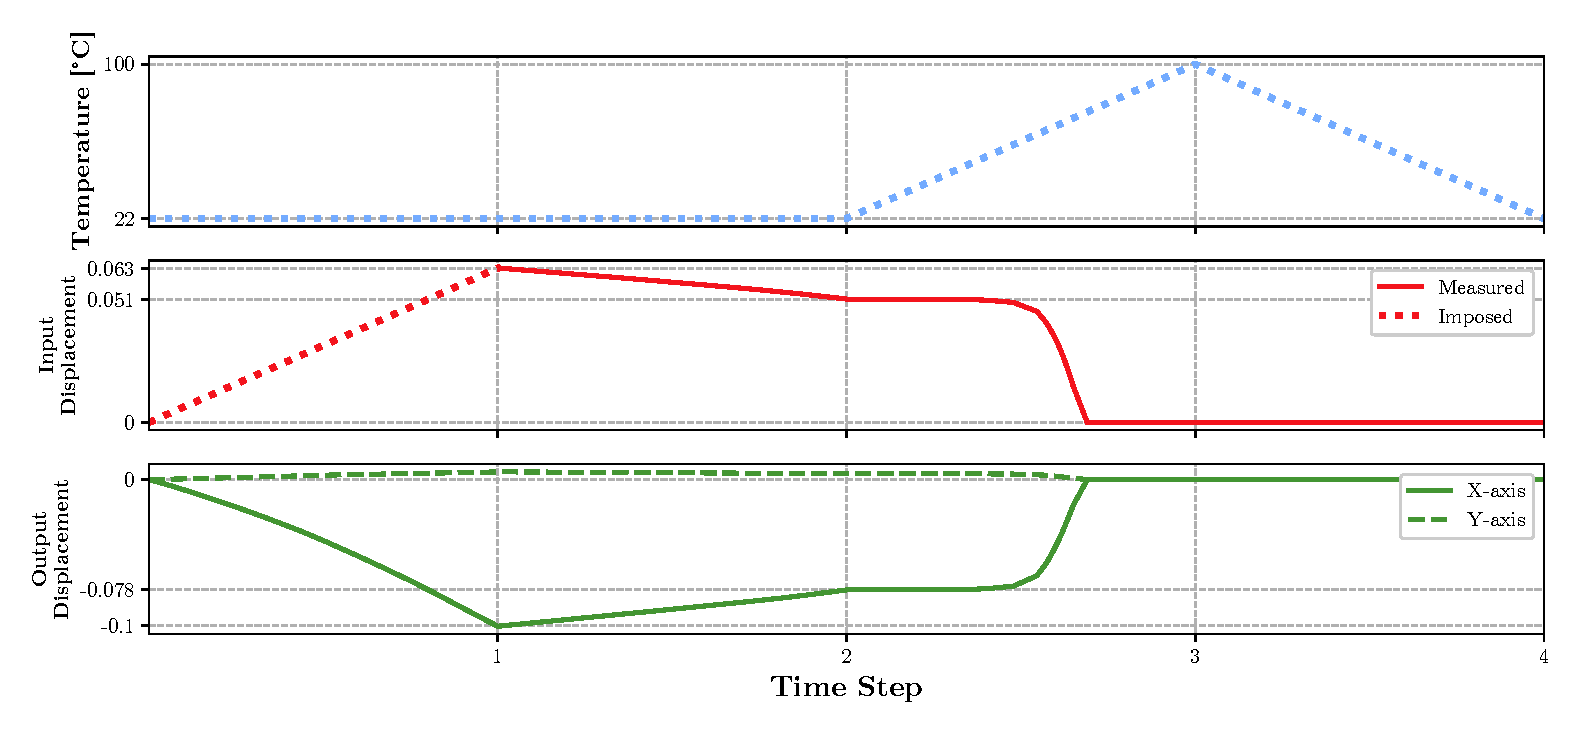
\includegraphics[width=\textwidth]{images/chap5/BM_Inverter30.eps}};
    \begin{scope}[x={(graph.south east)},y={(graph.north west)}]
    % \coordinate (ts0) at (1.54,7.6);
    % \coordinate (ts4) at (17.55,7.6);
    \coordinate (ts0) at (0.089,0.945);
    \coordinate (ts4) at (0.985,0.945);
    \coordinate (ts1) at ($ (ts0)!0.25!(ts4) $);
    \coordinate (ts2) at ($ (ts0)!0.5!(ts4) $);
    \coordinate (ts3) at ($ (ts0)!0.75!(ts4) $);
    \node[anchor=mid,inner sep=0] (ls0) at ($(ts0)!0.5!(ts1) + (0,0.05) $) {\fbox{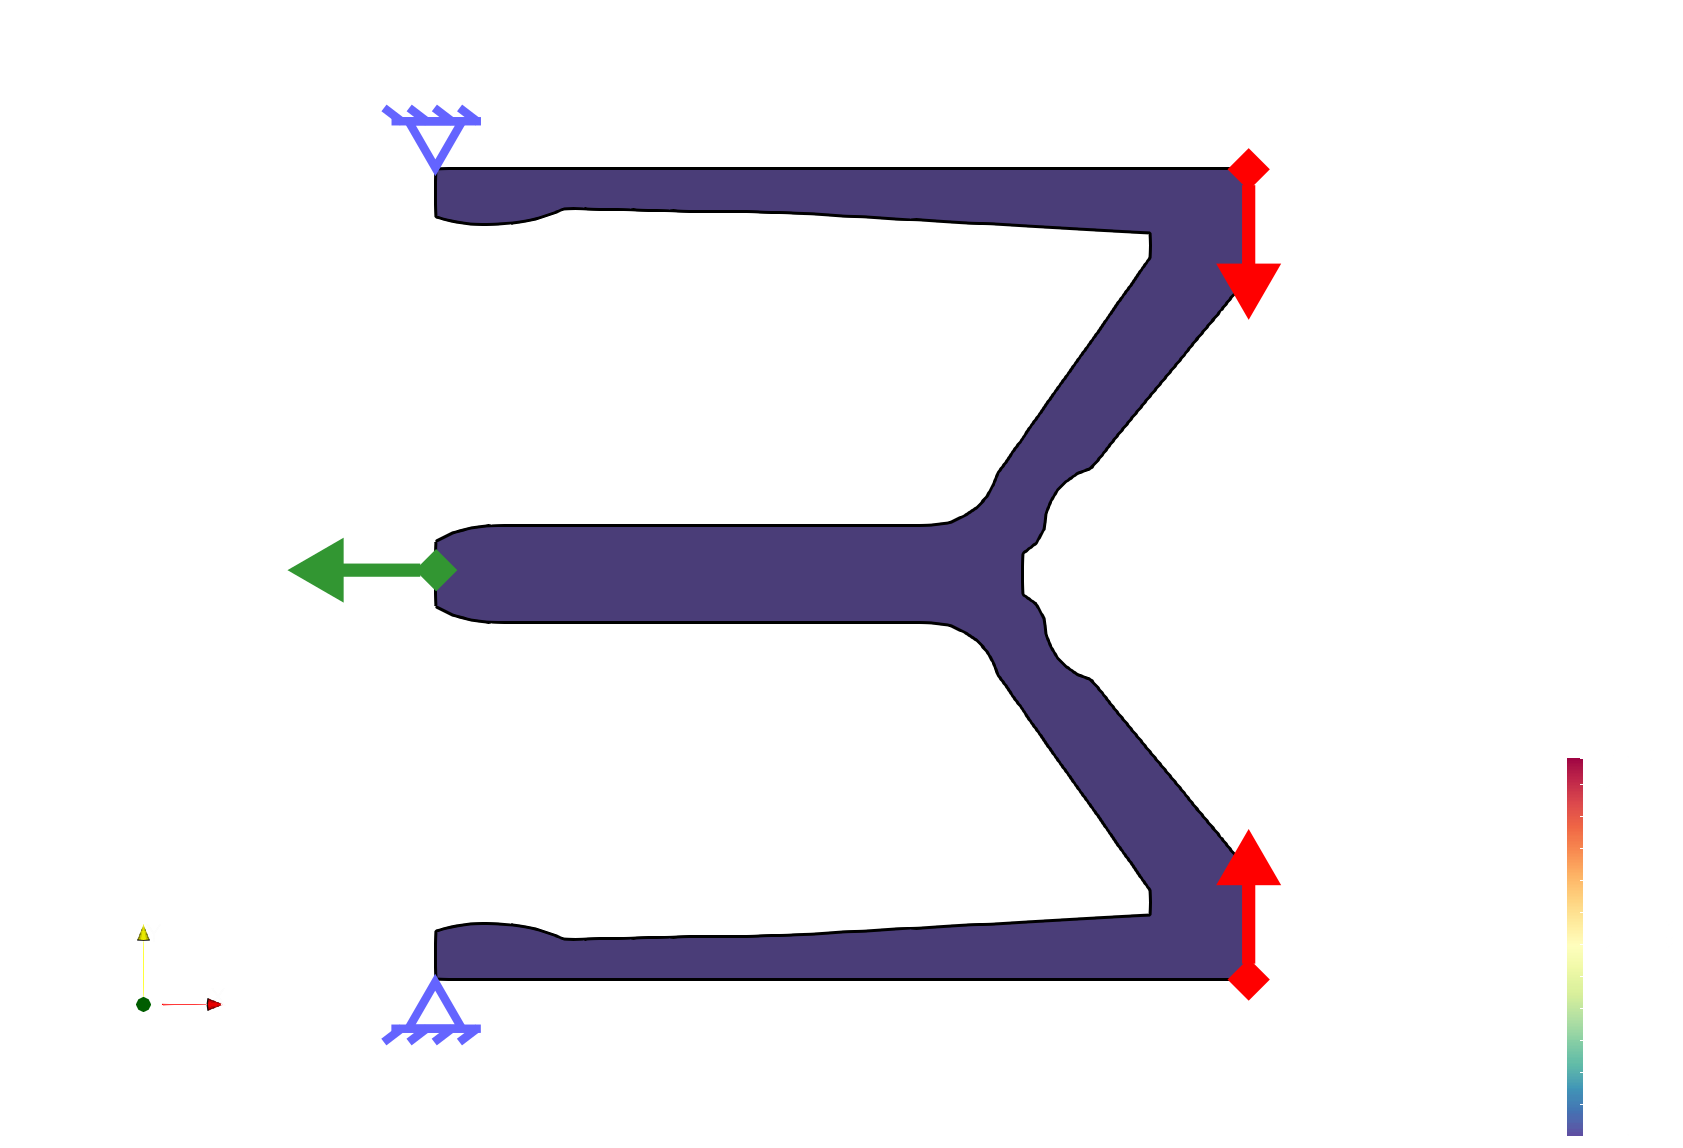
\includegraphics[height = 2cm,trim={11cm 3cm 13cm 3cm},clip]{images/chap5/Crimper_step0_v3.png}}};
    \draw[black, thick, -latex](ls0.west) to [bend right] (ts0);
    \node[anchor=mid,inner sep=0] (ls1) at ($(ts1)!0.5!(ts2) + (0,0.05) $) {\fbox{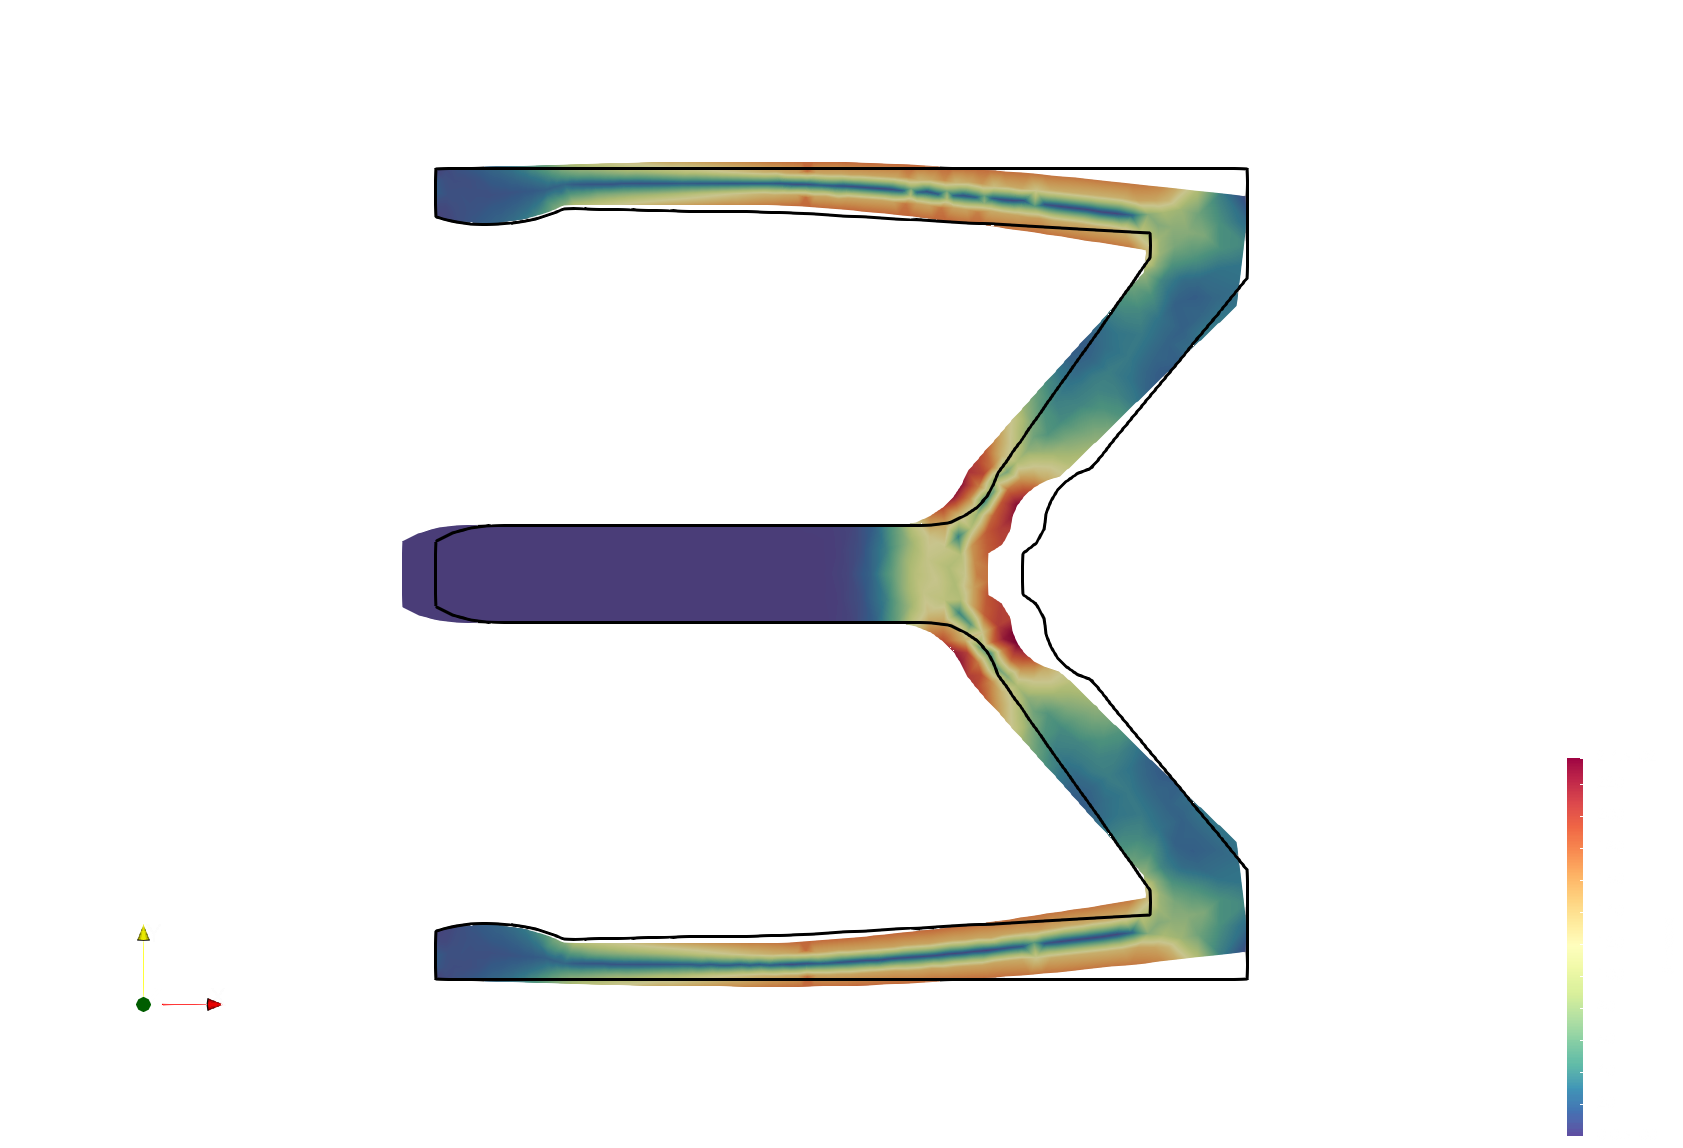
\includegraphics[height = 2cm,trim={11cm 3cm 13cm 3cm},clip]{images/chap5/Crimper_step1.png}}};
    \draw[black, thick, -latex](ls1.west) to [bend right] (ts1);
    \node[anchor=mid,inner sep=0] (ls2) at ($(ts2)!0.5!(ts3) + (0,0.05) $) {\fbox{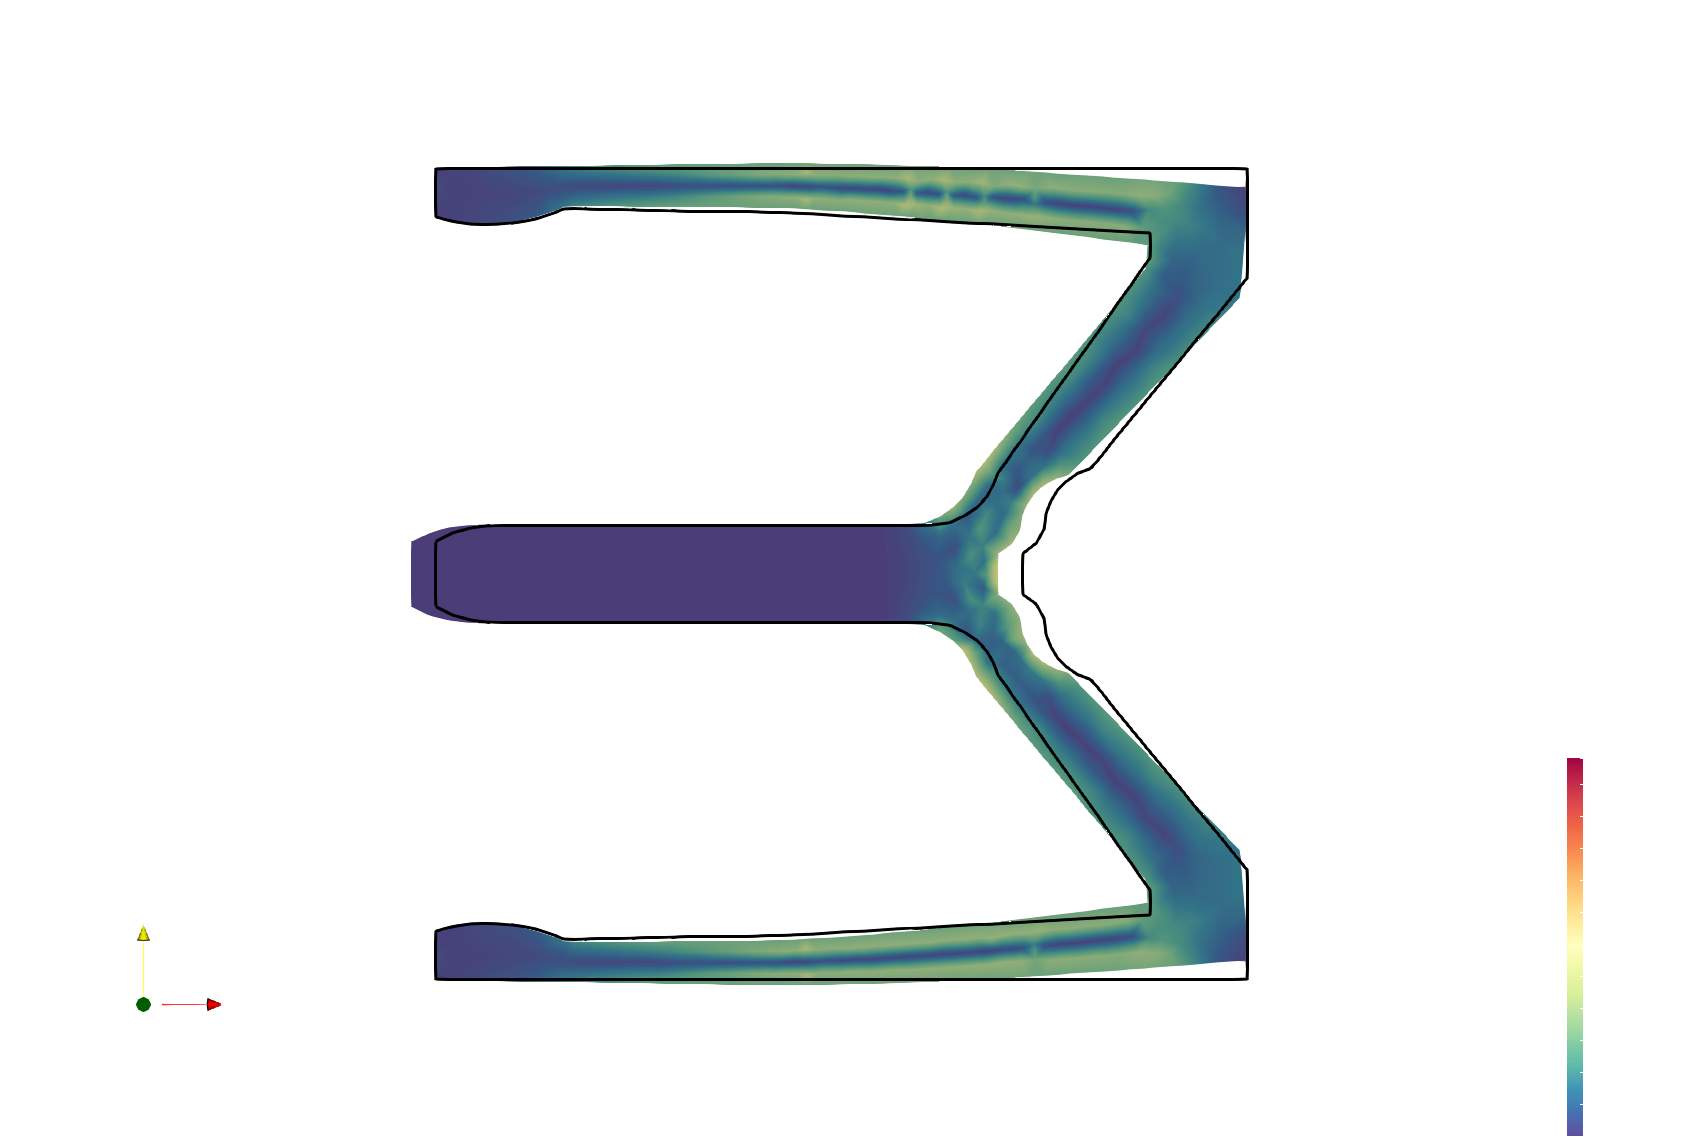
\includegraphics[height = 2cm,trim={11cm 3cm 13cm 3cm},clip]{images/chap5/Crimper_step2.png}}};
    \draw[black, thick, -latex](ls2.west) to [bend right] (ts2);
    \node[anchor=mid,inner sep=0] (ls3) at ($(ts3)!0.5!(ts4) + (0,0.05) $) {\fbox{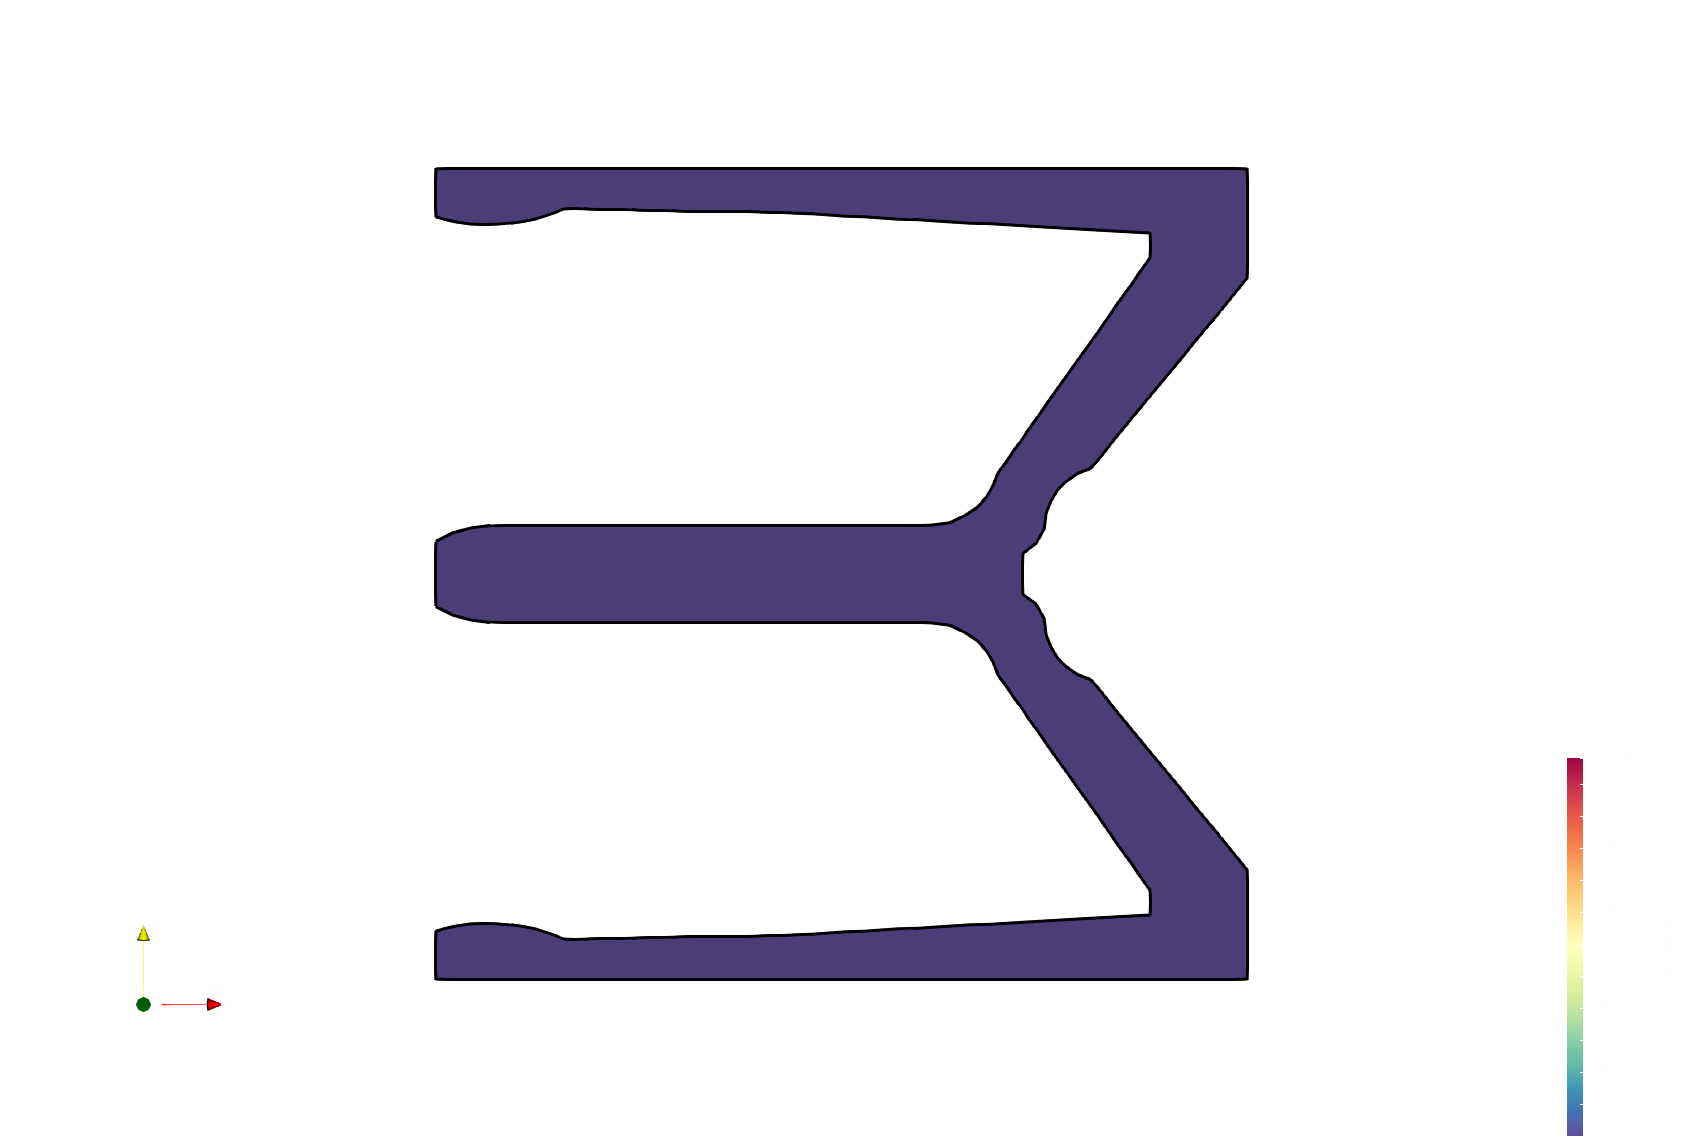
\includegraphics[height = 2cm,trim={11cm 3cm 13cm 3cm},clip]{images/chap5/Crimper_step0.png}}};
    \draw[black, thick, -latex](ls3.west) to [bend right] (ts3);
    \node[anchor=south east,inner sep=0] (ls0) at ($(ts4) + (0,0.015) $) {
\includegraphics[height = 2.3cm]{images/chap5/Colorbar.pdf}};
    \end{scope}
    \end{tikzpicture}%
\end{document}
